%\documentclass[conference]{IEEEtran}
%\IEEEoverridecommandlockouts
%\usepackage[english]{babel}

\documentclass[12pt]{article}
\usepackage[letterpaper,top=2cm,bottom=3cm,left=2cm,right=2cm,marginparwidth=1.75cm]{geometry}


% Set page size and margins
% Replace `letterpaper' with `a4paper' for UK/EU standard size

\usepackage{doi}
\bibliographystyle{apalike}

\usepackage{subcaption} 
\usepackage{enumitem}

\usepackage{graphicx}
\usepackage{amssymb}
\usepackage{amsmath}
\usepackage{dsfont}
\usepackage{xurl}

\usepackage{tikz}
\usetikzlibrary{arrows,automata,backgrounds,fit,patterns,petri,shadows,shapes}
\pgfdeclarepatternformonly{stripes}
{\pgfpointorigin}{\pgfpoint{0.25cm}{0.25cm}}
{\pgfpoint{0.25cm}{0.25cm}}
{
    \pgfpathmoveto{\pgfpoint{0cm}{0cm}}
    \pgfpathlineto{\pgfpoint{0.25cm}{0.25cm}}
    \pgfpathlineto{\pgfpoint{0.25cm}{0.12cm}}
    \pgfpathlineto{\pgfpoint{0.12cm}{0cm}}
    \pgfpathclose%
    \pgfusepath{fill}
    \pgfpathmoveto{\pgfpoint{0cm}{0.12cm}}
    \pgfpathlineto{\pgfpoint{0cm}{0.25cm}}
    \pgfpathlineto{\pgfpoint{0.12cm}{0.25cm}}
    \pgfpathclose%
    \pgfusepath{fill}
}

\usepackage{comment}
\usepackage{array}
\usepackage{booktabs}
\usepackage{bm}

\usepackage{hyperref}
\hypersetup{breaklinks=true,
    pdftitle={Optimal incentive schemes to enhance colorectal cancer screening participation}} 


\tikzstyle{decisionPM} = [rectangle, draw, thick, minimum size = 0.8cm, fill = green!20]
\tikzstyle{decisionC} = [rectangle, draw, thick, minimum size=0.8cm, fill = yellow!20]
\tikzstyle{decisionSP} = [rectangle, draw, thick, minimum size=0.8cm, fill = blue!20]
\tikzstyle{decisionF} = [rectangle, draw, thick, minimum size=0.8cm, fill = orange!20]
\tikzstyle{determ} = [circle, draw, thick, double, minimum size = 0.8cm]
\tikzstyle{chance} = [circle, thick, minimum size = 0.8cm, inner sep= 1pt, draw = black, pattern = stripes, pattern color = gray!40]
\tikzstyle{chanceD} = [circle, thick, minimum size = 0.8cm, inner sep= 1pt, draw = black]
\tikzstyle{chanceA} = [circle, thick, minimum size = 0.8cm, inner sep= 1pt, draw = black, fill = gray!40]


\tikzstyle{utilityPM} = [regular polygon, regular polygon sides = 6, draw, inner sep= 1pt, thick, minimum size=0.8cm, fill = green!20]
\tikzstyle{utilityC} = [regular polygon, regular polygon sides = 6, draw, inner sep= 1pt, thick, minimum size=0.8cm, fill = yellow!20]
\tikzstyle{utilitySP} = [regular polygon, regular polygon sides = 6, draw, inner sep= 1pt, thick, minimum size=0.8cm, fill = blue!20]
\tikzstyle{utilityF} = [regular polygon, regular polygon sides = 6, draw, inner sep= 1pt, thick, minimum size=0.8cm, fill = orange!20]
\tikzstyle{arrow} = [thick,->,>=stealth]


%\usepackage{cite}
\usepackage{amsmath,amssymb,amsfonts}
\usepackage{algorithmic}
\usepackage{graphicx}
\usepackage{textcomp}
\usepackage{xcolor}
\def\BibTeX{{\rm B\kern-.05em{\sc i\kern-.025em b}\kern-.08em
    T\kern-.1667em\lower.7ex\hbox{E}\kern-.125emX}}
\usepackage[round]{natbib}
\usepackage{enumitem}

\begin{document}

\title{Optimal incentive schemes to enhance colorectal cancer screening participation\thanks{Work supported by the AXA-ICMAT Chair in Adversarial Risk Analysis; the Spanish Ministry of Science project PID2021-124662OB-I00; the European Union's Horizon 2020 Research and Innovation Programme under Grant Agreement N. 101097036 (ONCOSCREEN); and the European Commission – NextGenerationEU, through the Momentum CSIC Programme: Develop Your Digital Talent}
}

%\author{\IEEEauthorblockN{Daniel Corrales}
%\IEEEauthorblockA{\textit{Mathematical Sciences Institute, ICMAT-CSIC}\\
%Madrid, Spain daniel.corrales@icmat.es}
%\and
%\IEEEauthorblockN{David Rios Insua}
%\IEEEauthorblockA{\textit{Mathematical Sciences Institute, ICMAT-CSIC}\\
%Madrid, Spain david.rios@icmat.es}
%}

%\author{Daniel Corrales \\
%ICMAT-CSIC \and David Rios Insua \\ ICMAT-CSIC}
\author{}
\date{ONGOING WORK WITHIN ONCOSCREEN PROJECT.\\ DO NOT CIRCULATE}

\maketitle
\begin{abstract}
Colorectal cancer (CRC) screening programmes in Europe reach far fewer citizens than they invite. We design incentive schemes to raise participation from the perspective of a policymaker who does not know the citizens' preferences and beliefs, using adversarial risk analysis to forecast how citizens, and a service provider delivering the programme, respond to incentives and contracts. We compare a public scheme, in which the policymaker offers a common incentive, with an outcome-based contract, under which a provider can also vary incentives across groups and navigate or support the access of citizens who do not respond. Applied to Spanish FIT screening, inviting citizens by assessed risk rather than age is a safe gain, and a common incentive a larger but less certain one, whose size depends on how strongly participation responds to money. The outcome-based contract improves on the public scheme only through access support, a lever a centrally run programme lacks, and only while that support is effective and affordable: without it, delegation costs the policymaker a rent and nothing else.
\end{abstract}

\begin{small}
\textbf{Keywords}: Colorectal cancer, screening, incentives, decision analysis, public-private partnerships.     
\end{small}



%%%%%%%%%%%%%%%%%%%%%%%%%%%%%%%%%%%%%%%%%%%%%%%%%
\section{Introduction}\label{intro}
 
Colorectal cancer (CRC) is the third most common type of cancer worldwide, making up about 10\% of all cancer cases \citep{WHO} and accounting for approximately 12\% of all cancer-associated deaths. In 2020, there were 1.9 million new cases and 930,000 associated deaths worldwide \citep{morgan2023global}. Just in the EU, its estimated annual costs in 2015 were approximately 19 B€ \citep{henderson2021economic}. Importantly, the societal costs associated with late-stage detection have proved higher than those related to early-stage detection \citep{mar2017cost}.

Despite this, only about 14\% of invited susceptible EU citizens participate in screening programmes, which currently mostly use one-size-fits-all strategies based on age and rely on fecal testing, which is cheap and comfortable but not highly accurate. If test results are positive, colonoscopy is recommended, which is very accurate but expensive, extremely uncomfortable, and even entails deadly risks. Hence, there is a need for: i) accurate, non-invasive, cost-effective screening tests based on novel technologies; ii) raising further awareness about the disease and the relevance of its early detection; iii) introducing personalised screening approaches covering genetic and socioeconomic factors as well as environmental stressors that potentially lead to different disease onsets; and iv) producing incentive schemes to increase participation in screening programmes, the subject of this paper.

The meta-analysis in \cite{facciorusso2021addition} concerning the impact of incentives to promote adherence to CRC screening programmes in the USA suggested a slightly positive impact, even though the incentives used were low. \cite{neuvonen2025optimizing} introduce a portfolio optimisation scheme to design screening programmes, including a yes/no decision concerning the introduction of a small (10€) scheme to promote participation. The approach we adopt here is different, as we aim at designing optimal incentives for a given screening procedure and compare various incentive mechanisms. The basic idea is that incentives can induce better adherence to a screening programme and, consequently, lead to earlier detection of CRC cases, thus increasing disease survival rates and improving quality of life among CRC patients, which can compensate for the incentive costs.

Many public policies use such incentives, and they must be designed with care: too large, they strain public budgets, as Spain's early subsidies to solar energy showed, having to be abruptly cancelled \citep{del2012support}; too small, they fail to change behaviour, as incentives of 5€ for CRC screening suggest \citep{facciorusso2021addition}.

The problem we therefore face is determining optimal financial incentives from the point of view of a policymaker (PM) taking into account the behaviour of the citizens (C).  In some of the schemes to be analysed, there will be a private third party, a designated service provider (SP), managing and implementing screening and incentives. In broad terms, the problem of designing incentives can be understood as a game and, more specifically, as a principal-agent problem \citep{smith1997principal} where the PM is the principal and the citizens are viewed as agents. For reasons outlined in \cite{rios2009adversarial} and \cite{ARAoverview}, rather than adopting standard game-theoretic approaches typical of this domain, relying on Nash equilibria and related refinements, we pursue a decision analytic approach based on adversarial risk analysis (ARA). This is a methodology to support a decision maker under uncertainty conditions in the presence of agents with different goals. In such a situation, the PM models the behaviour of the citizens to forecast their adherence and, accordingly, finds incentives that modify it. To showcase the flexibility of the methodology, we illustrate it with a purely {\em public scheme} involving two agents, and a public-private scheme involving three agents based on {\em outcome-based payments}.


Our contributions are threefold. First, we formulate incentive design for screening as an adversarial risk analysis problem, in which the PM forecasts participation from a random model of the citizens' preferences and beliefs rather than assuming common knowledge. Second, we extend it to an outcome-based contract with a service provider, a three-agent problem in which the PM forecasts the provider's campaign and the provider forecasts the citizens' responses. Third, we apply both to Spanish FIT screening, comparing age- and risk-based invitation, a common incentive, and a contract under which the provider can vary incentives across groups and navigate or support the access of citizens who do not respond, and we attribute the value of delegation to each of these levers. Section~\ref{sec:incentive_problem_definition} formulates both schemes, Section~\ref{sec:modelling_results} specifies and solves them, Section~\ref{sec:discussion} discusses the findings and their limitations, and Section~\ref{sec:conclusions} concludes.

  
For this, we draw on the database presented in Appendix \ref{app:models} as well as on earlier models for CRC prediction \citep{corrales2024colorectal} and screening \citep{corrales2025decision} summarised in the same appendix. Code to reproduce the models introduced here is available at \url{https://github.com/DanielCorralesAlonso/optimized_crc_incentives_ara}.

%%%%%%%%%%%%%%%%%%%%%%%%%%%%%%%%%%%%%%%%%%%%%%%%%%%%%%
\section{Incentives to increase screening participation} \label{sec:incentive_problem_definition}
Section \ref{sec:basic_setup} introduces the general problem setup, while Sections \ref{sec:public_scheme} and \ref{sec:OBP} define the theoretical framework for the public scheme and the public-private scheme, respectively.

%%%%%%%%%%%%%%%%%%%%%%%
\subsection{Basic setup} \label{sec:basic_setup}
A screening policy \emph{scr} assigns to each citizen with covariates $x$ a screening test, $scr(x)$, with a positive result being followed by a confirmatory colonoscopy, thereby defining the target population $\mathcal{T} = \{ i : scr(x_i) \neq \varnothing \}$ of citizens invited to screening. Policies range from one-size-fits-all rules based on age, as in most European organised programmes, to personalised rules based on the risk of having cancer given additional covariate information $p( c = 1 \mid x)$, possibly predicted by a model such as that in \cite{corrales2024colorectal}. As a personalised policy example, \cite{corrales2025decision} offer a stool-DNA (sDNA) test to citizens above a risk threshold $\xi_1$ and a fecal immunochemical test (FIT) for a risk between $\xi_2$ and $\xi_1$, assigning tests based on their reduction of disease uncertainty relative to their cost and comfort.

As a baseline policy, we adopt the standard age-based approach of organised programmes, offering a FIT test to every citizen in a target age band. We compare the baseline with a risk-based policy that offers FIT to the same number of citizens, those with the highest $p(c = 1 \mid x)$, whatever their age. Further, we distinguish different risk assessments made by different agents based on the information available to them. For example, a screening policy may be defined based on the policymaker's risk assessment $p_{PM}(c = 1 | x)$, while citizen participation may respond to their own risk assessment $p_C(c=1 | x)$. This distinction matters because the incentive generally acts on the gap between the two.

Even when screening is in the citizens' best interests, many do not attend, for reasons including lack of information, inappropriate communication, aversion to the screening methods, or misestimation of risk \citep{KASTRINOS}. We design two incentive schemes to raise participation, model each through a multi-agent influence diagram (MAID) \citep{banks2015adversarial}, and specify parametrisations under which they can be solved; Section~\ref{sec:modelling_results} solves them numerically.

%%%%%%%%%%%%%%%%%%%%%%%%%%%%%%%%
\subsection{A public scheme}\label{sec:public_scheme}
Consider first a mechanism consisting of the PM directly providing a target population $\mathcal{T}$ of identified citizens a financial incentive if they participate and complete the screening programme. This could take several forms, including, e.g., health insurance or tax reduction.

%%%%%%%%%%%%%%%%%%%%%%%%%%%%%%%%%%
\subsubsection{Modelling the public scheme through a bi-agent influence diagram}
The biagent influence diagram (BAID) in Figure \ref{fig:original_problem} captures the essence of the proposed incentive scheme. Green nodes correspond to the  $PM$, yellow nodes to $C$, and striped nodes are common to both agents.\footnote{Circles represent uncertainties, squares reflect decisions, and hexagons represent evaluations. Arcs pointing into decision nodes indicate that the corresponding decisions are made knowing the values of the parents. Arcs pointing to chance or value nodes indicate that, respectively, the predecessor values influence the corresponding probabilities or utilities.}
 
The chance variables involved are: the covariates $X$ of the citizens\footnote{In our case, for reasons described in \cite{corrales2024colorectal}, we include age, sex, socioeconomic situation, sleep duration, physical activity, depression, smoking, anxiety, alcohol consumption, body-mass index, hypercholesterolemia, diabetes, and hypertension.}; the citizen CRC status $c \in \{0,1\}$ (having $\{1\}$ or not $\{0\}$ the illness); the screening result $\mathcal{R} \in \{\varnothing, 0, 1\}$, taking values positive $\{1\}$, negative $\{0\}$ or null $\{\varnothing\}$, the latter arising when the citizen declines the invitation; the stage $G \in \{0, \text{I}, \text{II}, \text{III}, \text{IV}\}$, at which a cancer is diagnosed, which depends on whether it is detected by screening, with $G=0$ for no cancer; and the indicator $D \in \{0,1\}$ of death from CRC within five years, which depends on the stage. Finally, $\theta$ collects the uncertainty about the stage at diagnosis and about treatment costs. These are assumed to be common to all citizens, as opposed to $c$, $r$, $g$ and $d$, which are realised citizen by citizen. Importantly, striped chance nodes are said to be common to both agents but each of them might have their own subjective belief of their value, thus differentiating, e.g., $p_{PM}(c \mid x)$ and $p_{C}(c \mid x)$. The decision nodes are $\mathcal{S} \in \{0,1\}$, where 1 means the citizen accepts the screening invitation, and the incentive policy $\mathcal{I}$ offered by the PM to C if screening is completed. Finally, the value nodes $U_{\text{PM}}$ and $U_C$ correspond to the PM and C, respectively. % \cite{corrales2025decision} characterises and assesses the arcs involving screening results and their associated probabilities.

\begin{figure*}[h!]
    \centering
    % -----------------------------------------------------------
    % 1) ORIGINAL PROBLEM
    % -----------------------------------------------------------
    \begin{subfigure}[t]{0.32\textwidth}
        \centering
        \resizebox{\linewidth}{!}{%
        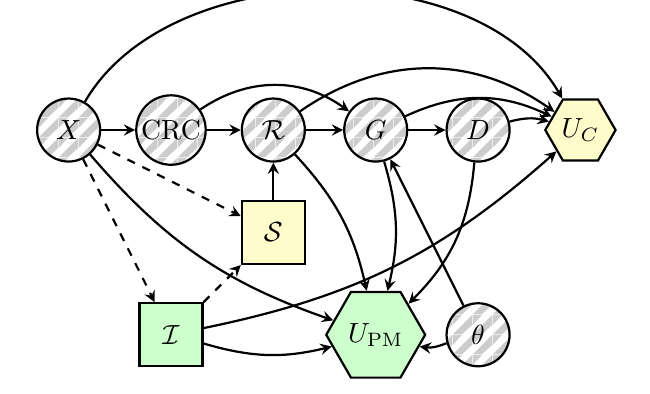
\begin{tikzpicture}[x=1.3cm, y=1.3cm]
            \useasboundingbox (-0.4, -1.3) rectangle (5.4, 2.0);
            
            % Nodes
            \node (ev)       at (0, 1)   [chance] {$X$};
            \node (crc)      at (1, 1)   [chance] {CRC};
            \node (res_scr)  at (2, 1)   [chance] {$\mathcal{R}$};
            \node (stage)    at (3, 1)   [chance] {$G$};
            \node (death)    at (4, 1)   [chance] {$D$};
            \node (util_cit) at (5, 1)   [utilityC] {$U_{C}$};
            \node (scr)      at (2, 0)   [decisionC] {$\mathcal{S}$};
            \node (I)        at (1, -1)  [decisionPM] {$\mathcal{I}$};
            \node (util_pm)  at (3, -1)  [utilityPM] {$U_{\text{PM}}$};
            \node (theta)    at (4, -1)  [chance] {$\theta$};

            % Disease and detection
            \draw [arrow] (ev) -- (crc);
            \draw [arrow] (crc) -- (res_scr);
            \draw [arrow] (scr) -- (res_scr);
            \draw [arrow, bend left=35] (crc) to (stage); 
            \draw [arrow] (res_scr) -- (stage);
            \draw [arrow] (stage) -- (death);
            
            % Information
            \draw [arrow, dashed] (ev) -- (I);
            \draw [arrow, dashed] (ev) -- (scr); 
            \draw [arrow, dashed] (I) -- (scr);

            % Into U_C (All Curved)
            \draw [arrow] (ev) to[out=60, in=120, looseness=0.9] (util_cit);
            \draw [arrow, bend left=35] (res_scr) to (util_cit); 
            \draw [arrow, bend left=25] (stage) to (util_cit);   
            \draw [arrow, bend left=15] (death) to (util_cit);
            \draw [arrow, bend right=15] (I) to (util_cit); 

            % Into U_PM (All Curved)
            \draw [arrow, bend right=15] (ev) to (util_pm); 
            \draw [arrow, bend left=15] (res_scr) to (util_pm); 
            \draw [arrow, bend left=15] (stage) to (util_pm);
            \draw [arrow, bend left=20] (death) to (util_pm);
            \draw [arrow, bend right=15] (I) to (util_pm);
            \draw [arrow, bend left=15] (theta) to (util_pm);
            
            \draw [arrow] (theta) -- (stage); % standard arc
        \end{tikzpicture}}
        \caption{CRC screening incentive problem}
        \label{fig:original_problem}
    \end{subfigure}
    \hfill
    % -----------------------------------------------------------
    % 2) PM'S PERSPECTIVE
    % -----------------------------------------------------------
    \begin{subfigure}[t]{0.32\textwidth}
        \centering
        \resizebox{\linewidth}{!}{%
        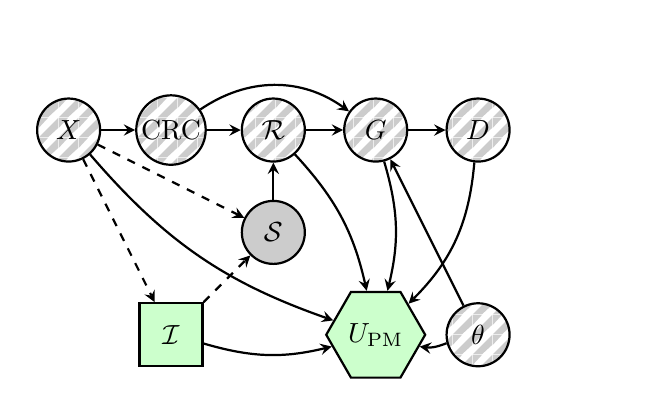
\begin{tikzpicture}[x=1.3cm, y=1.3cm]
            \useasboundingbox (-0.4, -1.3) rectangle (5.4, 2.0);
            
            \node (ev)       at (0, 1)   [chance] {$X$};
            \node (crc)      at (1, 1)   [chance] {CRC};
            \node (res_scr)  at (2, 1)   [chance] {$\mathcal{R}$};
            \node (stage)    at (3, 1)   [chance] {$G$};
            \node (death)    at (4, 1)   [chance] {$D$};
            \node (scr)      at (2, 0)   [chanceA] {$\mathcal{S}$};
            \node (I)        at (1, -1)  [decisionPM] {$\mathcal{I}$};
            \node (util_pm)  at (3, -1)  [utilityPM] {$U_{\text{PM}}$};
            \node (theta)    at (4, -1)  [chance] {$\theta$};

            \draw [arrow] (ev) -- (crc);
            \draw [arrow] (crc) -- (res_scr);
            \draw [arrow] (scr) -- (res_scr);
            \draw [arrow, bend left=35] (crc) to (stage);
            \draw [arrow] (res_scr) -- (stage);
            \draw [arrow] (stage) -- (death);
            
            \draw [arrow, dashed] (ev) -- (I);
            \draw [arrow, dashed] (ev) -- (scr);
            \draw [arrow, dashed] (I) -- (scr);

            % Into U_PM (All Curved)
            \draw [arrow, bend right=15] (ev) to (util_pm);
            \draw [arrow, bend left=15] (res_scr) to (util_pm);
            \draw [arrow, bend left=15] (stage) to (util_pm);
            \draw [arrow, bend left=20] (death) to (util_pm);
            \draw [arrow, bend right=15] (I) to (util_pm);
            \draw [arrow, bend left=15] (theta) to (util_pm);
            
            \draw [arrow] (theta) -- (stage);
        \end{tikzpicture}}
        \caption{PM's incentive problem}
        \label{fig:PM_problem}
    \end{subfigure}
    \hfill
    % -----------------------------------------------------------
    % 3) CITIZEN'S PERSPECTIVE
    % -----------------------------------------------------------
    \begin{subfigure}[t]{0.32\textwidth}
        \centering
        \resizebox{\linewidth}{!}{%
        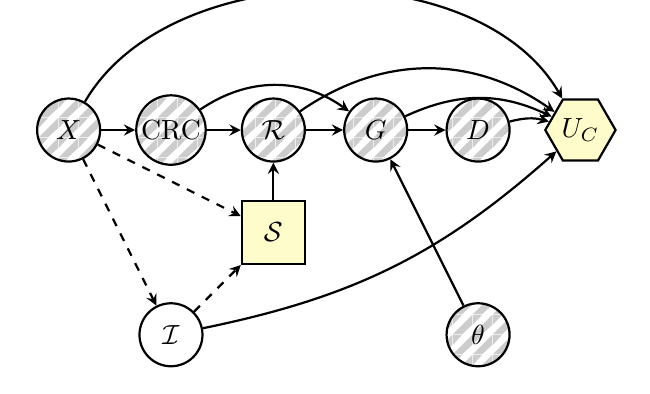
\begin{tikzpicture}[x=1.3cm, y=1.3cm]
            \useasboundingbox (-0.4, -1.3) rectangle (5.4, 2.0);
            
            \node (ev)       at (0, 1)   [chance] {$X$};
            \node (crc)      at (1, 1)   [chance] {CRC};
            \node (res_scr)  at (2, 1)   [chance] {$\mathcal{R}$};
            \node (stage)    at (3, 1)   [chance] {$G$};
            \node (death)    at (4, 1)   [chance] {$D$};
            \node (util_cit) at (5, 1)   [utilityC] {$U_{C}$};
            \node (scr)      at (2, 0)   [decisionC] {$\mathcal{S}$};
            \node (I)        at (1, -1)  [chanceD] {$\mathcal{I}$};
            \node (theta)    at (4, -1)  [chance] {$\theta$};

            \draw [arrow] (ev) -- (crc);
            \draw [arrow] (crc) -- (res_scr);
            \draw [arrow] (scr) -- (res_scr);
            \draw [arrow, bend left=35] (crc) to (stage);
            \draw [arrow] (res_scr) -- (stage);
            \draw [arrow] (stage) -- (death);
            
            \draw [arrow, dashed] (ev) -- (I);
            \draw [arrow, dashed] (ev) -- (scr);
            \draw [arrow, dashed] (I) -- (scr);

            % Into U_C (All Curved)
            \draw [arrow] (ev) to[out=60, in=120, looseness=0.9] (util_cit);
            \draw [arrow, bend left=35] (res_scr) to (util_cit);
            \draw [arrow, bend left=25] (stage) to (util_cit);
            \draw [arrow, bend left=15] (death) to (util_cit);
            \draw [arrow, bend right=15] (I) to (util_cit);
            
            \draw [arrow] (theta) -- (stage);
        \end{tikzpicture}}
        \caption{C's incentive problem}
        \label{fig:citizen_problem}
    \end{subfigure}

    \caption{BAIDs for the single citizen public scheme.}
    \label{fig:both_problems}
\end{figure*}


%%%%%%%%%%%%%%%%%%%%%%%%%%%%%%%%%%%%%
\subsubsection{Incentivising a single citizen}\label{sec:single_patient}
We first show how the PM sets the incentive for a single citizen with ARA, the basis for the population schemes that follow.
 %%%%%%%%%%%%%%%%%%%%%%%%%%%%%%%%%%%%%
\subparagraph{PM problem.} In our model, we weaken common knowledge assumptions typical of game theory; see, e.g.\ \cite{raiffa2007negotiation}.  The PM solves the decision analysis problem in Figure \ref{fig:PM_problem} by modelling C's screening decision with uncertainty $\pi_{PM}(s | \mathcal{I}, x)$, and also having probabilities about outcomes, $p_{PM}(c,r,g,d,\theta \mid s, \mathcal{I}, x)$, and their own utility function $u_{PM}(r,g,d,\mathcal{I},x, \theta)$. Given these, the PM's optimal incentive $\mathcal{I}^*(x)$ for a person with features $x$ is obtained as a solution to the maximum expected utility problem $\mathcal{I}^* (x)  =  \arg \max_{\mathcal{I}} \psi_{PM}(\mathcal{I}, x)$, where
\begin{align} \label{eq:max_util_PM}
  \psi_{PM}(\mathcal{I} , x) = & \quad \mathbb{E}_{\pi_{PM}(s \mid \mathcal{I}, x),\, p_{PM}(c,r,g,d,\theta \mid s, \mathcal{I}, x)} \big[u_{PM}(r,g,d,\mathcal{I},x, \theta)\big] \\
     = & \int \sum_{s} \sum_{r} \sum_{c} \sum_{g} \sum_{d} u_{PM}(r,g,d,\mathcal{I},x, \theta) \times \notag \\
    & \quad \times p_{PM}(c \mid x)\, p_{PM}(r \mid c,s)\, p_{PM}(g \mid c,r,\theta)\, p_{PM}(d \mid g)\, \pi_{PM}(s \mid \mathcal{I},x)\, p_{PM}(\theta) \, d\theta \notag
\end{align}
possibly subject to constraints such as a maximum budget or a cap on the incentive to individuals.

Except for $\pi_{PM}(s \mid \mathcal{I}, x)$, the ingredients in (\ref{eq:max_util_PM}) are standard in decision analysis terms \citep{french} (e.g. utility $u_{\text{PM}}$),  have been previously characterised (e.g. $p_{PM}(c \mid x)$ and $p_{PM}(r \mid c,s,scr)$ in \cite{corrales2024colorectal, corrales2025decision}), or will be described in the following sections ($p_{PM}(g \mid c,r,\theta)$, $p_{PM}(d \mid g)$ and $p_{PM}(\theta)$ in Section~\ref{sec:common_framework}). The remaining probability distribution $\pi_{PM}(s \mid \mathcal{I}, x)$ entails strategic thinking aspects that we now address, as it involves modelling C's problem from the perspective of the PM.

%%%%%%%%%%%%%%%%%%%%%%%%%%%%%%%%%%%
\subparagraph{Citizen's problem.} To assess such distribution, consider $C$'s problem (Figure \ref{fig:citizen_problem}) for a given $\mathcal{I}$ and $x$. Since the PM does not fully know $C$'s beliefs $p_C$ and preferences $u_C$, the solution requires modelling the PM's uncertainty about the citizen's utility and probability functions $(u_{C}, p_{C})$ through a random utility $U_C$ and a random distribution $P_C$ \citep{rios2009adversarial}, represented as $ F_C  \sim ( U_C, P_C )$. We call a single draw from $F_C$ a citizen \emph{type} $t$. This induces a distribution over the citizens' expected utility, defined through 
\begin{align}\label{eq:randexp}
    \Psi_C (s \mid \mathcal{I} , x) = & \quad \mathbb{E}_{P_{C}(c,r,g,d,\theta \mid s, x)} \big[U_C(r,g,d,\mathcal{I},x, \theta) \big]  \\
    = & \int \sum_{r} \sum_{c} \sum_{g} \sum_{d} U_C(r,g,d, \mathcal{I},x,\theta) \times \nonumber \\
     & \qquad  \times \, P_C(c \mid x)\, P_C(r \mid c,s)\, P_C(g \mid c,r,\theta)\, P_C(d \mid g)\, P_C(\theta) \, d\theta. \nonumber
\end{align}
The PM then estimates the required probabilities through
\begin{align}\label{eq:probPM}
    \pi_{PM}(s \mid \mathcal{I}, x) = \mathbb{P}_{F_C}\big[\arg \max_{s' \in \{0,1\}} \Psi_C (s' \mid \mathcal{I} , x) = s\big].
\end{align}
Computationally, we draw $N_C$ types $t^{(n)} \sim F_C$, $n = 1, \dots, N_C$ and find
\begin{align*}
    s_{n}^*(\mathcal{I} , x) = \arg \max_{s} \int \sum_{r,c,g,d} U_C^{t^{(n)}}(r,g,d,\mathcal{I},x,\theta) \, P_C^{t^{(n)}}(c \mid x)\, P_C^{t^{(n)}}(r \mid c,s)\, P_C^{t^{(n)}}(g \mid c,r,\theta)\, P_C^{t^{(n)}}(d \mid g)\, P_C^{t^{(n)}}(\theta) \, d\theta,
\end{align*}
and estimate the required probabilities through $\pi_{PM}(s \mid \mathcal{I}, x) \approx \# \{ n : s_n^*(\mathcal{I} , x) = s\} \big/ N_C$. These probabilities are then input into Equation~(\ref{eq:max_util_PM}) to determine $\mathcal{I}^* (x)$.


%%%%%%%%%%%%%%%%%%%%%%%%%%%%%%%%%%%%%%%%%%%%%
\subsubsection{Incentivising the entire population}\label{sec:incent}

\begin{figure}[h!]
    \centering
    \resizebox{0.5\linewidth}{!}{%
    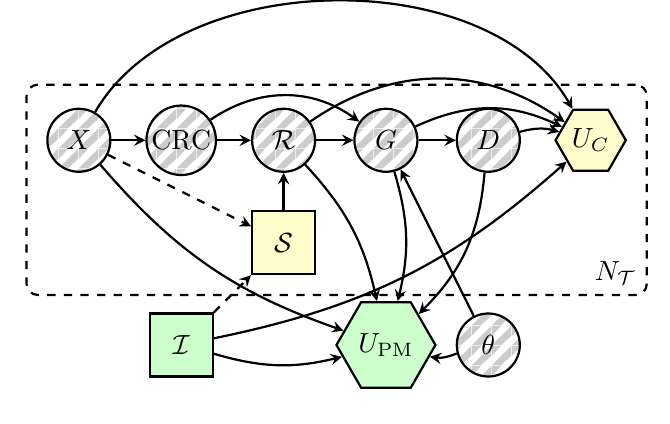
\begin{tikzpicture}[x=1.3cm, y=1.3cm]
        \useasboundingbox (-0.5, -1.5) rectangle (5.5, 2.1);
        
        % 1. CITIZEN LAYER (inside the plate)
        \node (ev)       at (0, 1)   [chance] {$X$};
        \node (crc)      at (1, 1)   [chance] {CRC};
        \node (res_scr)  at (2, 1)   [chance] {$\mathcal{R}$};
        \node (stage)    at (3, 1)   [chance] {$G$};
        \node (death)    at (4, 1)   [chance] {$D$};
        \node (util_cit) at (5, 1)   [utilityC] {$U_{C}$};
        \node (scr)      at (2, 0)   [decisionC] {$\mathcal{S}$};
        
        % 2. COMMON TO THE POPULATION (outside the plate)
        \node (I)        at (1, -1)  [decisionPM] {$\mathcal{I}$};
        \node (util_pm)  at (3, -1)  [utilityPM] {$U_{\text{PM}}$};
        \node (theta)    at (4, -1)  [chance] {$\theta$};
        
        % 3. THE PLATE
        \begin{scope}[on background layer]
            \node [draw, thick, rectangle, rounded corners, dashed,
                   fit=(ev) (crc) (util_cit) (scr),
                   inner sep=0.25cm,
                   label={[anchor=south east, inner sep=4pt]south east:$N_{\mathcal{T}}$}] (plate) {};
        \end{scope}
        
        % 4. ARROWS inside the plate
        \draw [arrow] (ev) -- (crc);
        \draw [arrow, dashed] (ev) -- (scr);
        \draw [arrow] (crc) -- (res_scr);
        \draw [arrow] (scr) -- (res_scr);
        \draw [arrow, bend left=35] (crc) to (stage);
        \draw [arrow] (res_scr) -- (stage);
        \draw [arrow] (stage) -- (death);
        
        % Into U_C (All curved)
        \draw [arrow] (ev) to[out=60, in=120, looseness=0.9] (util_cit);
        \draw [arrow, bend left=35] (res_scr) to (util_cit);
        \draw [arrow, bend left=25] (stage) to (util_cit);
        \draw [arrow, bend left=15] (death) to (util_cit);
        
        % 5. ARROWS crossing the plate into U_PM (All Curved)
        \draw [arrow, bend right=15] (ev) to (util_pm);
        \draw [arrow, bend left=15] (res_scr) to (util_pm);
        \draw [arrow, bend left=15] (stage) to (util_pm);
        \draw [arrow, bend left=20] (death) to (util_pm);
        
        % 6. ARROWS from the common nodes
        \draw [arrow, dashed] (I) -- (scr);
        \draw [arrow] (theta) -- (stage);
        
        % From common nodes to utilities (All curved)
        \draw [arrow, bend right=15] (I) to (util_cit);
        \draw [arrow, bend right=15] (I) to (util_pm);
        \draw [arrow, bend left=15] (theta) to (util_pm);
    \end{tikzpicture}}
    \caption{Incentivising the entire population with a common incentive.}
    \label{fig:common_incentive_problem}
\end{figure}

Most currently active public programmes are designed so that the incentive is common for all citizens within the target population \citep{facciorusso2021addition}. Let $\mathcal{T}$ be the target population composed of $N_{\mathcal{T}}$ citizens with corresponding covariates $\mathbf{x} = (x_i)_{i=1}^{N_\mathcal{T}}$, and designate with $\mathbf{s}, \mathbf{c}, \mathbf{r}, \mathbf{g}, \mathbf{d}$ the corresponding vectors of decisions, CRC statuses, results, stages, and CRC deaths. The PM now seeks $\mathcal{I}^{*} = \arg \max_{\mathcal{I}} \psi_{PM}(\mathcal{I}; \mathcal{T})$, where
\begin{align}\label{eq:expected_util_population}
 \psi_{PM}&(\mathcal{I} ; \mathcal{T})
  = \mathbb{E}_{\pi_{PM}(\mathbf{s} \mid \mathcal{I}, \mathcal{T}),\, p_{PM}(\mathbf{c}, \mathbf{r}, \mathbf{g}, \mathbf{d}, \theta \mid \mathbf{s}, \mathcal{I}, \mathcal{T})} \big[u_{PM}( \mathbf{r}, \mathbf{g}, \mathbf{d}, \mathcal{I}, \mathbf{x}, \theta)\big] \\
  & \qquad \ \ = \int   p_{PM}(\theta)\, \bigg[ \sum_{\mathbf{s}} \sum_{\mathbf{r}} \sum_{\mathbf{c}} \sum_{\mathbf{g}} \sum_{\mathbf{d}}
     u_{PM}\big( \mathbf{r}, \mathbf{g}, \mathbf{d}, \mathcal{I}, \mathbf{x}, \theta \big) \times \notag\\
  &\quad  \times
     \prod_{i=1}^{N_{\mathcal{T}}}
        p_{PM}(c_i\mid x_i)\, p_{PM}(r_i\mid c_i, s_i, scr(x_i))\, p_{PM}(g_i \mid c_i, r_i, \theta)\, p_{PM}(d_i \mid g_i)\, \pi_{PM}(s_i\mid\mathcal{I}, x_i) \bigg]\, d\theta. \notag
\end{align}
As we now cover a whole set of citizens, the sums in Equation~(\ref{eq:expected_util_population}) run over a space growing exponentially in $N_{\mathcal{T}}$ and are never evaluated directly. Note that $\theta$ lies outside the product as, given $\theta$, citizens are independent, but $\theta$ itself is shared by all of them. For a general utility $u_{\text{PM}}$, the expectation must be taken by simulation. A value $\theta \sim p_{PM}(\theta)$ is drawn; replicates of the entire population outcome are then drawn given it, with $c_i \sim p_{PM}(c \mid x_i)$, $s_i \sim \pi_{PM}(s \mid \mathcal{I}, x_i)$, $r_i \sim p(r \mid c_i, s_i, scr(x_i))$, $g_i \sim p(g \mid c_i, r_i, \theta)$ and $d_i \sim p(d \mid g_i)$ for each citizen; $u_{\text{PM}}$ is evaluated once per replicate and averaged over replicates and draws of $\theta$. This simulation pipeline is detailed in Appendix~\ref{app:simulation_public}.

Every replicate requires $\pi_{PM}(s \mid \mathcal{I}, x_i)$, and hence a solution of the citizen's problem, for every relevant $(\mathcal{I}, x)$. Since the citizen's problem depends on $x$ only through the age group, the assigned test and the citizen's own risk assessment $p_C(c \mid x)$, it is solved once per covariate profile, and the same draws of the citizen type serve every incentive. The optimisation for $\mathcal{I}^*$ may be done by fitting a surrogate model $\widehat{\psi}_{PM}(\mathcal{I})$ on the grid $\{(\mathcal{I}_k, \psi_{PM}(\mathcal{I}_k ; \mathcal{T}))\}_{k=1}^{|\mathbb{I}|}$, e.g.\ through a Gaussian process \citep{gramacy2020surrogates}. Common random numbers are used across the incentive grid and across draws of $\theta$.


 
%%%%%%%%%%%%%
\subsection{Outcome based payments}\label{sec:OBP}
The private-public scheme studied here is \emph{outcome-based payments (OBP)}, described in detail in \cite{vlaanderen2019design} and \cite{fox2021evaluating}. In these financial models, payment is tied to the outcomes achieved rather than to the mere delivery of a service or product; {\em pay-for-performance} schemes are the closest established variant, and {\em value-based payment} is often used interchangeably, although the latter term is broader. One example in the health sector is the {\em Best Practice Tariffs} model of the English NHS \citep{kristensen2016optimal}.

In this type of scheme, besides the agents PM and C of Section~\ref{sec:single_patient}, a third actor appears: a service provider (SP) which delivers screening on behalf of the PM. Delegation is attractive because the SP can do what a centrally run programme cannot: it can vary incentives across population groups, contact non-responders in person, and help them take and return the test. That same capacity is, however, effort the PM cannot observe, namely whom the SP contacts, how, and with what inducement, so the PM pays for observable outcomes instead. The OBP scheme thus reimburses the SP conditionally on meeting predefined screening and detection targets.\footnote{An independent auditor verifies the reported outcomes. Its role is what renders those outcomes contractible in the first place, but it is passive as regards incentive design, and we leave it, and its cost, outside the model.}

OBPs may adopt numerous parametric forms. To fix the discussion, we use one comprising a payment for the care delivered and two further payments conditional on what the campaign achieves. The SP receives from the PM the aggregation of
\begin{itemize}
    \item {\em Base payment} (BP). Reimbursement, at the PM's unit prices, of the care delivered: the tests analysed and the confirmatory colonoscopies performed.
    \item {\em Outcome payment}. An amount of up to $z_4$ € per invited citizen, earned as coverage rises from a lower threshold $z_2$ to an upper threshold $z_1$: nothing is earned when less than a fraction $z_2$ of the target population is screened, the full amount at or above $z_1$, and a proportional share in between.
    \item {\em Bonus}. An additional payment of $z_3$ € per CRC case confirmed through the screening pathway.
\end{itemize}
Let us write $\mathcal{O}$ for the audited screening record of the campaign, from which follow the cost $BP(\mathcal{O})$ of the care delivered, the fraction $q(\mathcal{O})$ of the target population screened, and the number $n(\mathcal{O})$ of CRC cases confirmed. The contract then pays
\begin{align}\label{eq:obp}
  obp(\mathcal{O}, z) = BP(\mathcal{O}) + z_4\, N_{\mathcal{T}}\, \omega\big(q(\mathcal{O}); z_1, z_2\big) + z_3\, n(\mathcal{O}),
  \qquad
  \omega(q; z_1, z_2) = \min\!\left\{ \max\!\left\{ \frac{q - z_2}{z_1 - z_2},\, 0 \right\},\, 1 \right\},
\end{align}
with $z = (z_1, z_2, z_3, z_4)$ in $Z = \{ z : 0 \leq z_2 < z_1 \leq 1,\ z_3 \geq 0,\ z_4 \geq 0 \}$. The outcome payment has the shape of the \emph{Quality and Outcomes Framework} \citep{campbell2009effects}, a price per point scaled by list size and by achievement between two thresholds; its continuity means that small changes in coverage never change the payment discontinuously. Other shapes, such as steps, fit the framework unchanged.

The three payments focus on three distinct events: a test delivered, a population covered, and a case confirmed. The base payment reimburses the care delivered, but neither the invitations nor the incentives nor any other effort of the SP; these are financed from the outcome payment and the bonus, which is what makes the contract outcome-based. Coverage is measured against the whole target population rather than against those approached, so a threshold cannot be met by approaching fewer citizens. The four parameters separate the two roles a contract must fill: $z_1$ and $z_2$ fix the coverage over which the outcome payment is earned, while $z_4$ and $z_3$ fix what the PM pays for coverage and per case confirmed. We designate this scheme $obp(z)$, $z \in Z$.



%%%%%%%%%%%%%%%%%
\subsubsection{Modelling OBPs through a multi-agent influence diagram}
The OBP scheme adopts the MAID structure in Figure~\ref{fig:multiagent_obp}. Blue nodes refer to the SP, with green and yellow denoting PM and C, respectively, as in the public scheme. The citizen nodes are those of Figure~\ref{fig:common_incentive_problem}.

\begin{figure}[h!]
    \centering
    \resizebox{0.65\linewidth}{!}{%
    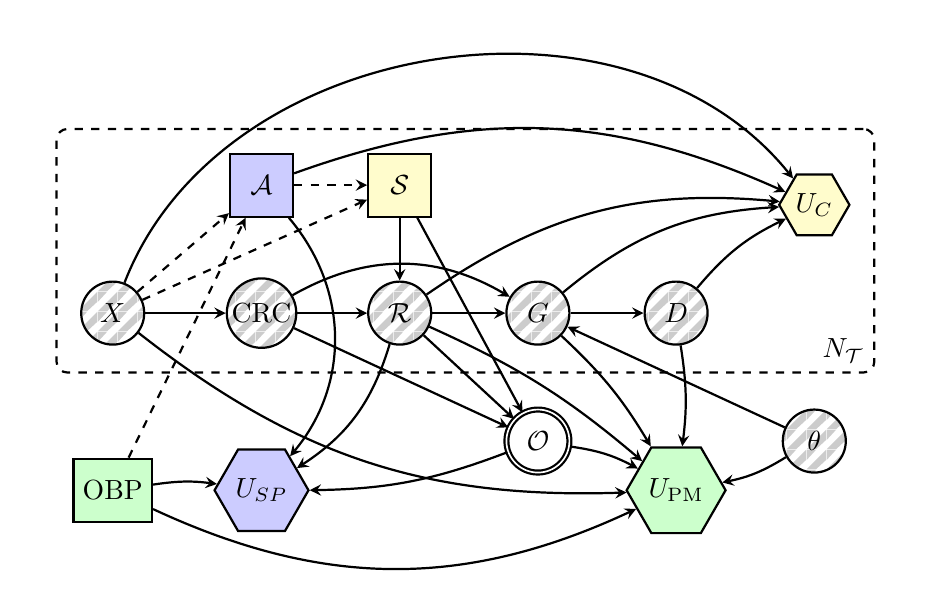
\begin{tikzpicture}[x=1.35cm, y=1.25cm]
        \useasboundingbox (-0.8, -2.4) rectangle (7.4, 3.2);
        % 1. DECISIONS (top), CITIZEN CHAIN (middle)
        \node (ev)       at (0, 0.3)     [chance]     {$X$};
        \node (A)        at (1.4, 1.6)   [decisionSP] {$\mathcal{A}$};
        \node (scr)      at (2.7, 1.6)   [decisionC]  {$\mathcal{S}$};
        \node (crc)      at (1.4, 0.3)   [chance]     {CRC};
        \node (res_scr)  at (2.7, 0.3)   [chance]     {$\mathcal{R}$};
        \node (stage)    at (4.0, 0.3)   [chance]     {$G$};
        \node (death)    at (5.3, 0.3)   [chance]     {$D$};
        \node (util_cit) at (6.6, 1.4)   [utilityC]   {$U_{C}$};
        % 2. COMMON NODES (outside the plate)
        \node (theta)    at (6.6, -1)  [chance]     {$\theta$};
        \node (detected) at (4.0, -1)  [determ]     {$\mathcal{O}$};
        \node (OBP)      at (0, -1.5)    [decisionPM] {OBP};
        \node (util_sp)  at (1.4, -1.5)  [utilitySP]  {$U_{SP}$};
        \node (util_pm)  at (5.3, -1.5)  [utilityPM]  {$U_{\text{PM}}$};
        % 3. THE PLATE
        \begin{scope}[on background layer]
            \node [draw, thick, rectangle, rounded corners, dashed,
                   fit=(ev) (A) (scr) (crc) (util_cit),
                   inner sep=0.3cm,
                   label={[anchor=south east, inner sep=4pt]south east:$N_{\mathcal{T}}$}] (plate) {};
        \end{scope}
        % 4. CHANCE ARCS (straight)
        \draw [arrow] (ev) -- (crc);
        \draw [arrow] (crc) -- (res_scr);
        \draw [arrow] (scr) -- (res_scr);
        \draw [arrow, bend left=30] (crc) to (stage);
        \draw [arrow] (res_scr) -- (stage);
        \draw [arrow] (stage) -- (death);
        \draw [arrow] (theta) -- (stage);
        % 5. INFORMATION ARCS (dashed, into decisions)
        \draw [arrow, dashed] (ev) -- (A);
        \draw [arrow, dashed] (ev) -- (scr);
        \draw [arrow, dashed] (A) -- (scr);
        \draw [arrow, dashed] (OBP) -- (A);
        % 6. AUDITED RECORD (straight, into a deterministic node)
        \draw [arrow] (crc) -- (detected);
        \draw [arrow] (scr) -- (detected);
        \draw [arrow] (res_scr) -- (detected);
        % 7. VALUE ARCS (curved, into utilities)
        \draw [arrow, bend left=12] (death) to (util_cit);
        \draw [arrow, bend left=18] (stage) to (util_cit);
        \draw [arrow, bend left=20] (res_scr) to (util_cit);
        \draw [arrow, bend left=22] (A) to (util_cit);
        \draw [arrow, bend left=60] (ev) to (util_cit);
        \draw [arrow, bend left=40] (A) to (util_sp);
        \draw [arrow, bend left=20] (res_scr) to (util_sp);
        \draw [arrow, bend left=10] (detected) to (util_sp);
        \draw [arrow, bend left=8]  (OBP) to (util_sp);
        \draw [arrow, bend right=25] (OBP) to (util_pm);
        \draw [arrow, bend right=20] (ev) to (util_pm);
        \draw [arrow, bend left=8]  (res_scr) to (util_pm);
        \draw [arrow, bend left=8]  (stage) to (util_pm);
        \draw [arrow, bend left=8]  (death) to (util_pm);
        \draw [arrow, bend left=10] (detected) to (util_pm);
        \draw [arrow, bend left=10] (theta) to (util_pm);
    \end{tikzpicture}}
    \caption{MAID for the OBP scheme. The dashed plate replicates the citizen subproblem over the $N_{\mathcal{T}}$ citizens of the target population; $\theta$, the contract, the audited record $\mathcal{O}$ and the value nodes of the PM and the SP lie outside it.}
    \label{fig:multiagent_obp}
\end{figure}
A realisation $a_i = (\mathcal{I}(x_i), \ell(x_i))$ of the decision $\mathcal{A}$ for citizen $i$ combines the incentive offered with the support the citizen receives should they not respond to the invitation, $\ell_i = (\ell_i^{N}, \ell_i^{A}) \in \{0,1\}^2$, indicating navigation and access support. The campaign $\mathbf{a} = (a_i)_{i \in \mathcal{T}}$ is a plan fixed before invitations are sent, and every citizen in $\mathcal{T}$ is invited, as organised programmes must invite their whole eligible population. Through the arc $X \dashrightarrow \mathcal{A}$, the SP may condition the plan on the citizens' covariates.

The node $\mathcal{O}$ records the number of citizens screened, the number of positive screening results, the number of CRC cases confirmed after colonoscopy, and the cost of the care delivered. These are the quantities entering $BP$, $q$ and $n$ in \eqref{eq:obp}.

The rounded box denotes replication of the citizen subproblem over the $N_{\mathcal{T}}$ individuals of the target population. It does not, however, mean independence, as $\mathcal{O}$ aggregates all citizens' subproblems, so the coverage tiers are evaluated jointly on the whole target population, and the SP values its global position rather than each citizen separately. Therefore, its optimisation does not decompose across individuals, in contrast to the per-citizen treatment of Section~\ref{sec:single_patient}. 

Decision-making hence proceeds as follows:
\begin{itemize}
    \item The PM designs the scheme, in our case fixing $z$, by modelling how the SP will run the campaign and how citizens will respond to it.

    \item The SP, observing $z$, fixes its campaign, modelling how citizens will react to it.

    \item Citizens are asked to decide whether to participate or not. Those who accept are assumed to complete the programme, and the incentive is paid. A positive result calls for a confirmatory colonoscopy, which establishes the citizen's CRC status and enters them into the corresponding care pathway. Those who do not respond may receive navigation or access support under the SP's plan and decide again.

    \item Outcomes are audited through $\mathcal{O}$ and the PM pays the SP according to $obp(\mathcal{O}, z)$.

    \item The PM assesses the programme's global results with the type of results reflected in  Table~\ref{tab:comparison}.
\end{itemize}


%%%%%%%%%%%%%%%%%%%%%%%%%
\subsubsection{Solution approach}\label{sec:OBP_inc}
Similar to the public scheme, the PM requires modelling the other agents' problems to find its optimal contract design. 
\subparagraph{Citizen's problem.}
It is that of Section~\ref{sec:single_patient}, with the offer now made by the SP. The SP must now forecast the response, so the random model $F_C \sim (U_C, P_C)$ describing a citizen of unknown type is held by the SP and yields, for a citizen with covariates $x$ offered $a = (\mathcal{I}, \ell)$,
\begin{align} \label{eq:psi_C}
    \Psi_C&(s \mid a, x)
    = \mathbb{E}_{P_C(c \mid a, x)\, P_C(r \mid c, s, scr(x))\, P_C(g \mid c, r, \theta)\, P_C(d \mid g)\, P_C(\theta)}
       \big[ U_C( r, g, d, a, x ) \big]  \\
    &= \int \sum_{c,r,g,d}
       U_C( r, g, d, a, x )\,
       P_C(c \mid a, x)\, P_C(r \mid c, s, scr(x))\, P_C(g \mid c, r, \theta)\, P_C(d \mid g)\, P_C(\theta) \, \mathrm{d}\theta. \notag
\end{align}
The campaign reaches the citizen through three channels: the incentive enters their payoff, as in the public scheme; navigation acts on $P_C(c \mid a, x)$, their assessment of their own risk; and access support acts on $U_C$ through the burden of the test. The SP's forecast of acceptance is then
\begin{align} \label{eq:p_s}
    \pi_{SP}(s \mid a, x) = \mathbb{P}_{F_C}\!\left[
    \arg\max_{s'} \Psi_C(s' \mid a, x) = s \right].
\end{align}
The PM observes neither the campaign nor the SP's model of the citizen, and must represent both in turn.

%%%%%%%%%%%%%%%%%%%%%%%%%%%%%%%%%%%%%%%%%%%%%%%
\subparagraph{SP problem.}
Observing the contract $z$, the SP chooses a campaign $\mathbf{a}$, determining what each citizen is offered and which non-responders receive further support. The SP evaluates its global position under a utility $u_{SP}$, so its objective is
\begin{align}\label{eq:sp_util}
  \psi_{SP}(\mathbf{a} \mid z, \mathcal{T}) &= \mathbb{E}_{\pi_{SP}(\mathbf{s} \mid \mathbf{a}, \mathcal{T})\, p_{SP}(\mathbf{c}, \mathbf{r} \mid \mathbf{s}, \mathcal{T})} \big[ u_{SP}( \mathbf{a}, \mathbf{r}, \mathcal{O}, z ) \big] \\
  &= \sum_{\mathbf{s}} \sum_{\mathbf{c}} \sum_{\mathbf{r}}
    u_{SP}( \mathbf{a}, \mathbf{r}, \mathcal{O}, z )
    \prod_{i = 1}^{N_{\mathcal{T}}}
      p_{SP}(c_i \mid x_i)\, \pi_{SP}(s_i \mid a_i, x_i)\, p_{SP}(r_i \mid c_i, s_i, scr(x_i)), \notag
\end{align}
where $\mathcal{O}$ is determined by $(\mathbf{c}, \mathbf{r}, \mathbf{x})$. The contract pays on counts, so neither $\theta$ nor the stage and survival of citizens enter the SP's problem. The SP adopts the campaign of maximum expected utility
\begin{align}\label{eq:sp_argmax}
  \mathbf{a}^{*} = \arg\max_{\mathbf{a}}
    \psi_{SP}(\mathbf{a} \mid z, \mathcal{T}).
\end{align}
Note that the SP is already one level of an ARA recursion, and the PM now applies a second-level ARA step to the SP in turn, as the PM does not observe the SP's choice. In that sense, the PM uses a random model for the SP, denoted as $F_{SP} \sim  (U_{SP}, P_{SP})$, where $U_{SP}$ carries the PM's uncertainty about the SP's preferences and costs, and $P_{SP}$ carries its beliefs, including the citizen model $F_C$ on which $\pi_{SP}$ rests. This translates to modelling the SP objective as a random function $\Psi_{SP}(\mathbf{a} \mid z, \mathcal{T})$, and hence its maximiser is a random action. The PM's forecast assigns to each campaign the probability that it is the SP's choice,
\begin{align} \label{eq:sp_forecast}
    \pi_{PM}(\mathbf{a} \mid z, \mathcal{T})
    = \mathbb{P}_{F_{SP}}\!\left[\, \arg\max_{\mathbf{a}'}
        \Psi_{SP}(\mathbf{a}' \mid z, \mathcal{T}) = \mathbf{a} \,\right].
\end{align}

\subparagraph{PM problem.}
The PM needs to choose the OBP scheme, which amounts to choosing the parameters $z$ based on its expected utility function
\begin{align}\label{eq:pm_util}
    \psi_{PM}&(z \mid \mathcal{T}) = \mathbb{E}_{\pi_{PM}(\mathbf{a} \mid z, \mathcal{T})\, \pi_{PM}(\mathbf{s} \mid \mathbf{a}, \mathbf{x})\, p_{PM}(\mathbf{c}, \mathbf{r}, \mathbf{g}, \mathbf{d}, \theta \mid \mathbf{s}, \mathbf{x})} \big[ u_{PM}( \mathbf{r}, \mathbf{g}, \mathbf{d}, \mathbf{x}, \theta, \mathcal{O}, z) \big] \\
    & \qquad \ \ = \int p_{PM}(\theta) \bigg[ \sum_{\mathbf{a}} \sum_{\mathbf{s}} \sum_{\mathbf{r}} \sum_{\mathbf{c}} \sum_{\mathbf{g}} \sum_{\mathbf{d}}
     u_{PM}( \mathbf{r}, \mathbf{g}, \mathbf{d}, \mathbf{x}, \theta, \mathcal{O}, z)\, \pi_{PM}(\mathbf{a} \mid z, \mathcal{T}) \times \nonumber \\
    & \ \times \prod_{i=1}^{N_{\mathcal{T}}} p_{PM}(c_i \mid x_i)\, p_{PM}(r_i \mid c_i, s_i, scr(x_i))\, p_{PM}(g_i \mid c_i, r_i, \theta)\, p_{PM}(d_i \mid g_i)\, \pi_{PM}(s_i \mid a_i, x_i) \bigg]\,  \, d\theta. \notag
\end{align}
The PM's utility values the health outcomes and bears the contractual payment $obp(\mathcal{O}, z)$, with $\mathcal{O}$ determined by the realised outcomes. The SP's campaign enters through the single factor $\pi_{PM}(\mathbf{s} \mid \mathbf{a}, \mathbf{x})$, which influences what the PM values as it changes who accepts screening. The contract parameters act one step further back, through $\pi_{PM}(\mathbf{a} \mid z, \mathcal{T})$, as the PM cannot choose the campaign but only the terms under which the SP chooses it; assessing that factor is the PM's strategic step. The remaining factor, $\pi_{PM}(s_i \mid a_i, x_i)$, is the PM's own forecast of citizen acceptance, with the offer $a_i$ in place of the incentive $\mathcal{I}$, so that the lever enters the citizen's beliefs as it does in Equation (\ref{eq:psi_C}). It need not coincide with $\pi_{SP}(s_i \mid a_i, x_i)$; in the application the SP holds the PM's citizen model, handed over by the contract, so the two coincide.

As in Section~\ref{sec:incent}, a general $u_{\text{PM}}$ does not let the expectation factorise, and the shared block of $\theta$ couples the citizens. Here, a further expectation over the SP's campaign sits on top. We therefore proceed by simulation, following the scheme in Appendix~\ref{app:simulation_OBP_utility}. Choosing a grid $\mathcal{G} = \{z_m\}_{m=1}^{M} \subset Z$, we estimate $\psi_{PM}(z_m \mid \mathcal{T})$ at each point and take the maximiser $z^{*}$; the grid is checked against $z^*$ on every component, the natural bounds $z_1 = 1$ and $z_3 = 0$ being limits of the contract rather than of the grid. The resulting $obp(z^{*})$ is assessed in the same accounts as the public scheme (Table~\ref{tab:comparison}).


%%%%%%%%%%%%%%%%%
\begin{comment}
\subsection{Social impact bond}
Social impact bonds (SIBs), also known as {\em pay-for-success} contracts constitute an innovative financing mechanism designed to fund social programmes through partnerships between the public sector, private investors, and service providers. They are detailed in  \cite{berndt2018market}, \cite{fraser2018narratives}, and \cite{OECD}.

In a SIB, the SP becomes a mere service provider (it just delivers screening as required, with no targets entailing benefits), and there is a new actor, FUND, which bears the risk in search for a bigger screening goal possibly by investing through incentives, who would get a reimbursment from the PM in a similar fashion than in an OBP.  A SIB can adopt a parametric scheme similar to an OBP and, for the purpose of this discussion, we adopt that in Section \ref{sec:OBP}, with FUND replacing SP as payment receiver, and FUND finally paying the eventual screening costs to SP. We designate such scheme $sib(z)$ with, again, $z = (z_1, z_2, z_3 )$, and $ z_1 > z_2$. 

%%%%%%%%%%%%%%%%%
\subsubsection{Modelling SIBs through a multi-agent influence diagram}

Let us use the MAID in Figure \ref{fig:multiagent_sib}. In this case, brown nodes belong to FUND, who invests through incentives to achieve a better social outcome of a bigger proportion of the population at-risk screened. The new nodes in brown refer to FUND implementing the service and its utility function. We remove the SP nodes for clarity, as it is a mere service provider.

\begin{figure}[h!]
    \centering
    
        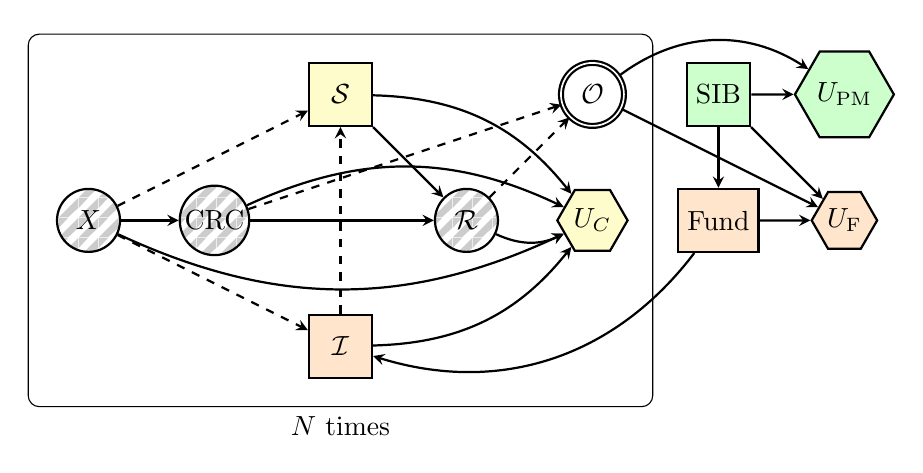
\begin{tikzpicture}[ node distance=1.6cm]
        
            % Nodes
            \node (ev) [chance] {$X$};
            \node (crc) [chance, right of=ev] {CRC};
            \node (scr) [decisionC, right of=crc, above of=crc] {$\mathcal{S}$};
            \node (I) [decisionF, below of =crc, right of =crc] {$\mathcal{I}$};
            \node (res_scr) [chance, right of=scr, below of = scr] {$\mathcal{R}$};
            %\node (util_sp) [utilitySP, below of = I] {$U_{\textit{SP}}$};
            \node (util_cit) [utilityC, right of = res_scr] {$U_{C}$};
            \node (detected) [determ, right of = I, above of = res_scr]{$\mathcal{O}$};
            \node (SIB) [decisionPM, right of = detected]{SIB};
            \node (util_pm) [utilityPM, right of = SIB] {$U_{\text{PM}}$};
            \node (Funding) [decisionF, below of = SIB]{Fund};
            \node (util_f) [utilityF, below of = util_pm] {$U_{\text{F}}$};
            
             
            % Arrows (influences)
            \draw [arrow] (ev) -- (crc);
            \draw [arrow, dashed] (ev) -- (scr);
            \draw [arrow, dashed] (I) -- (scr);
            \draw [arrow, dashed] (ev) -- (I);
            %\draw [arrow, dashed] (crc) -- (scr);
            %\draw [arrow, dashed] (crc) -- (I);
            \draw [arrow] (scr) -- (res_scr);
            \draw [arrow] (crc) -- (res_scr); 
            %\draw [arrow] (I) to (util_sp);
            \draw [arrow, dashed] (res_scr) to (detected);
            \draw [arrow, dashed] (crc) to (detected);
            %\draw [arrow] (detected) to (util_sp);
            \draw [arrow] (SIB) to (util_pm);
            \draw [arrow] (SIB) to (Funding);
            \draw [arrow] (SIB) to (util_f);
            \draw [arrow] (Funding) to (util_f);
            
            %\draw [arrow, bend right = 10] (ev) to (util_sp);
            %\draw [arrow, bend left = 30] (scr) to (util_sp); 
            %\draw [arrow, bend right = 5] (crc) to (util_sp);
            %\draw [arrow, bend left = 25] (res_scr) to (util_sp);
            \draw [arrow, bend right = 25] (ev) to (util_cit);
            \draw [arrow, bend right = 25] (I) to (util_cit);
            \draw [arrow, bend left = 25] (scr) to (util_cit);
            \draw [arrow, bend left = 25 ] (crc) to (util_cit);
            \draw [arrow, bend right = 25] (res_scr) to (util_cit);
            \draw [arrow] (detected) to (util_f);
             \draw [arrow, bend left = 35] (detected) to (util_pm);
            \draw [arrow, bend left = 35] (Funding) to (I);

            \node[draw, rectangle, rounded corners, fit=(ev)(scr)(I)(detected), inner sep=10pt] (groupA) {};
            \node at (groupA.south) [below] {$N$ times};
    
        \end{tikzpicture}
        \caption{Social impact bond as a multi-agent influence diagram}
        \label{fig:multiagent_sib}

    
\end{figure}

\noindent The decision making protocol would run now as follows:
 \begin{itemize}
 \item The PM designs a SIB, fixing $z$, taking into account (predicting) how FUND will promote the screening programme implementation and how the citizens will respond to such promotion.
 \item FUND decides about the incentivised programme to accompany the screening programme. 
 \item SP provides the screening services, which are called upon by FUND making use of the incentives
 delivered by FUND.
 \item The incumbent citizens receive the call to participate in the screening programme, including the incentive information, and decide whether or not to adhere to it. If they fully adhere, they receive the incentive. Eventually, their CRC status is predicted and a treatment decision is made.
 \item Once the programme has been implemented, its outcomes are assessed,\footnote{Again, typically undertaken 
  by an independent auditor. For modelling simplicity, we do not include them but take into account the corresponding costs.} PM pays FUND for the outcomes, and FUND pays 
   SP for the services.
 \end{itemize}



%%%%%%%%%%%%%%%%%%%%%%%%%
\subsubsection{Solution approach}

The SIB solution approach follows a similar path to that of the OBP (Section 2.3.2) with the following differences:
\begin{itemize}
    \item The specific problem of SP is not necessary, as it is merely a service provider with predefined service level agreements. For that reason, we did not display the corresponding nodes in Figure \ref{fig:multiagent_sib}.
    \item The FUND problem is similar to the SP problem in Section \ref{sec:OBP}. Again, the PM will know only partially the FUND judgements, modelled through random preferences and beliefs. Importantly, we would expect here the utility function  $u_F$ to be risk-prone (and the random utility function $U_F$ to have support over risk-prone utility functions).
    \item The citizen problem adopts a similar form to estimate $\pi_{PM}(s | I, x)$. We expect a larger number of communication attempts from FUND in this case, as well as a better-informed citizen, in the sense of receiving a less uncertain $p_C(c|x)$.
    \item The PM problem would adopt the same expression.
\end{itemize}
\end{comment}




%%%%%%%%%%%%%%%%%%%%%%%%%%%%%%%%%%%%%%%%%%%%
\section{Modelling and results} \label{sec:modelling_results}
We now specify the models of Section~\ref{sec:incentive_problem_definition} for Spanish FIT screening and solve them. Section~\ref{sec:public_scheme_modelling} specifies the valuation of outcomes and the citizen and PM models shared by both schemes, Section~\ref{sec:public_scheme_results} solves the public scheme, Section~\ref{sec:obp_modelling} specifies and solves the outcome-based payment, and Section~\ref{sec:comparison} compares the two. Parameters are taken from published sources when available; the remaining ones are stated as assumptions and examined in the sensitivity analyses. The parametric models are instrumental and may be replaced in other settings.
%%%%%%%%%%%%%%%%%%%%%%%%%%%%%%%%%%%
\subsection{Model specification} \label{sec:public_scheme_modelling}
We assume the PM has access to a CRC risk model, such as the one sketched in Appendix \ref{app:models}, so they are accurately informed of the probabilities $p_{PM}(c \mid x)$. Citizens are assumed to hold their own, possibly distorted, risk assessment $p_C(c \mid x)$. Several literature reviews point to a lack of information and risk misconception as one of the main reasons for low participation in screening programmes; see, e.g., \cite{wee2005factors}, \cite{le2023exploring}, or \cite{berg2022reasons}. 
 
Both schemes are evaluated on the records of the 2016 medical database described in Appendix \ref{app:models}, which covers $339{,}707$ citizens. The PM's $p_{PM}(c=1 \mid x)$ is given by a risk model evaluated on all the covariates in the records, while the citizen's $p_{C}(c=1 \mid x)$ is given by the same risk model evaluated only on a small subset of them, those a citizen can be expected to know and read as risk factors. Two policies select the target population $\mathcal{T}$, both offering the standard \emph{fecal immunochemical test} (FIT). The \emph{age-based} policy invites all $N_{\mathcal{T}} = 49{,}074$ citizens aged 60--69, the oldest band of the 50--69 programmes run in Spain. The \emph{risk-based} policy invites the same number of citizens with the highest $p_{PM}(c=1 \mid x)$, of whom 10{,}940 (22.3\%) are younger than 60. The citizen model is calibrated on the age-based policy and held fixed across policies (Section~\ref{sec:citizen_model}), so uptake differs between them only because they invite different citizens. Section~\ref{sec:common_framework} specifies how outcomes are valued, and Sections~\ref{sec:citizen_model} and~\ref{sec:pm_model} the citizen and PM models. The main structural assumptions are a single screening round, full adherence once a citizen accepts, stage distributions and mortality observed at ages 60--69 applied to every age group, a citizen model identified by a single calibrated moment, and risk-neutral PM and SP; Section~\ref{sec:discussion} discusses their consequences.

\subsubsection{Common framework}\label{sec:common_framework}
Common to both agents are the horizon over which health accrues and the health consequences of CRC and of screening, together with their uncertainty about them. 
\paragraph{Valuing health.} Assume that PM and C value health outcomes in monetary terms, pricing \emph{quality-adjusted life years} (QALYs) at the Spanish cost-effectiveness threshold of $v = 30{,}000$€ per QALY, consistent with Spanish Health Technology Assessment practice \citep{vallejo2018estimating, sacristan2002que}. Further, assume that a citizen with covariates $x$, in age group $a(x)$, has a \emph{remaining life expectancy} $\bar{Y}(a(x))$, and each of those life-years is quality-adjusted by the EQ-5D utility $u(a(x))$ of the age group \citep{garcia2016normative} (Table \ref{tab:age_stratified}). Health accrues as a stream over the years a citizen survives, and we write $A(Y,\lambda) = \big(1-(1+\lambda)^{-Y}\big)/\lambda$ for the present value at rate $\lambda$ of one unit per year over $Y$ years. Each agent applies its own rate. The PM discounts health at the social rate $\lambda_{PM} = 0.03$, a convention in Spanish HTA \citep{lopez2010spanish}, and citizens at their own $\lambda_C$.


\paragraph{CRC stage and survival.} We assume that a citizen without CRC survives the whole horizon, $Y = \bar{Y}(a(x))$. For a citizen with CRC, what screening changes is the stage $g \in \{\text{I}, \dots, \text{IV} \}$ at which the cancer is diagnosed, with $g = 0$ denoting no cancer. A cancer detected by screening ($r=1$) has stage distribution $\boldsymbol{\phi}^{\text{scr}}$; one missed by the test ($r=0$) or never screened ($r = \varnothing$) is eventually detected clinically, with distribution $\boldsymbol{\phi}^{\text{cli}}$:
\begin{equation}\label{eq:stage}
p(g \mid c, r, \theta) =
\begin{cases}
\mathbb{I}_{\{g = 0\}}, & c = 0,\\
\phi^{\text{scr}}_g, & c = 1,\ r = 1,\\
\phi^{\text{cli}}_g, & c = 1,\ r \neq 1.
\end{cases}
\end{equation}
Given the stage, the citizen dies of cancer within five years ($d=1$) with probability $\delta_g$, with $\delta_0 = 0$, regardless of how cancer was detected. Citizens surviving this period are treated as cured, and all deaths are placed at the middle of the five-year window, $t_D=2.5$ years, as if spread evenly over it, so that
\begin{equation}\label{eq:qdeath}
p(d = 1 \mid c, r, \theta) = \sum_{g} p(g \mid c, r, \theta)\, \delta_g,
\qquad
Y(d,x) = \bar Y(a(x))\,(1 - d) + t_D\, d .
\end{equation}
are the probability of death and the years survived. The health stream is then worth
\begin{equation}\label{eq:vfuture}
V^{j}_{\text{future}}(d, x) = v \cdot u(a(x)) \cdot A\big(Y(d,x), \lambda_j\big).
\end{equation}
A cancer thus kills with probability $\bar\delta_{\text{scr}} = \boldsymbol{\phi}^{\text{scr}} \cdot \boldsymbol{\delta}$ if detected by screening and $\bar\delta_{\text{cli}} = \boldsymbol{\phi}^{\text{cli}} \cdot \boldsymbol{\delta}$ otherwise. Since death shortens the stream of health from $\bar Y(a(x))$ to $t_D$ years, the loss scales with remaining life.

\paragraph{Treatment and health loss.} Cancer and its treatment also reduce quality of life while they last. A cancer diagnosed at stage $g$ lowers utility by $\Delta u_g(x)$ during the first $T_g$ years after diagnosis, with $\Delta u_0 = 0$, which is worth
\begin{equation}\label{eq:vtreat}
V^{j}_{\text{treat}}(g, x) = v \cdot \Delta u_g(x) \cdot A(T_g,\lambda_j)
\end{equation}
to an agent $j$ discounting at rate $\lambda_j$. From the meta-analysis of \citet{djalalov2014review}, utilities elicited three months after surgery are 0.05 lower than those elicited more than a year after it, and utilities at stage IV are a further 0.19 lower than at stages I--III. These decrements are elicited on populations whose reference utility is $0.90$, so we apply them in proportion to the citizen's own health state, taking $\Delta u_g(x) = 0.05\,u(a(x))/0.90$ for $T_g = 1$ year at stages I--III, and $\Delta u_{\text{IV}}(x) = 0.24\,u(a(x))/0.90$ until death, $T_{\text{IV}} = t_D$. The decrement applies whether or not the citizen survives the cancer and is borne by both agents (Table~\ref{tab:death_prob}).

We use external survival data to set the quantities we just defined. Among citizens aged 60--69, \citet{cardoso2022overall} report the stage distribution at diagnosis, with 43\% of screen-detected cancers at stage I against 19\% of those detected otherwise, and five-year overall survival $S_g$ by stage. Removing other-cause mortality, $\delta_g = 1 - S_g/S_0$, with $S_0 = l_{70}/l_{65} = 0.9528$ the five-year survival from other causes at these ages \citep{ine2024mortalidad}. At the reported stage distributions, $\bar\delta_{\text{scr}} = 0.224$ and $\bar\delta_{\text{cli}} = 0.381$. These figures refer to ages 60--69 and are applied to every age group.

\paragraph{Complications.} Screening has one further effect on health, which is the possible complications arising from colonoscopy. These include procedural complications, such as perforation or bleeding, and procedure-related deaths \cite{reumkens2016post, lin2021screening, barre2020cost}. These are measured as an expected loss $L_{COL}$ in QALYs, not temporally discounted as they are incurred within weeks of the test. We take it as procedure-related mortality, 2.9 per 100{,}000 colonoscopies \citep{reumkens2016post}, which at the discounted quality-adjusted life expectancy of a citizen aged 60--69, 14.04 QALYs, gives $L_{COL} = 4.07 \times 10^{-4}$ QALY. Perforation (0.5 per 1{,}000) and bleeding (2.6 per 1{,}000) enter through the cost of their treatment, included in $c_{col}$ (Table~\ref{tab:pm_params}); their loss of quality of life, being short-lived, is neglected.

\paragraph{Common knowledge.} The probability of each result, $p(r \mid c, s, scr(x))$, follows from the sensitivity and specificity of the assigned test (Table~\ref{tab:screening_tests}). These are taken as properties of the test rather than of the citizen, common and known to both agents. Likewise, $p(g \mid c, r, \theta)$ and $p(d \mid g)$ are common to both agents.

\paragraph{Outcome uncertainty.} Two kinds of uncertainty remain. Whether a given citizen has CRC, tests positive, is diagnosed at a given stage, and dies of the cancer is realised citizen by citizen, independently given the model parameters, and averages out over a large population. Those parameters themselves are uncertain and common to all citizens, so we collect them in $$ \theta = \big(\boldsymbol{\phi}^{\text{scr}}, \boldsymbol{\phi}^{\text{cli}}, \boldsymbol{\tau}\big),$$  where $\boldsymbol{\tau} = (\tau_{\text{I}}, \dots, \tau_{\text{IV}})$ denotes the treatment costs by stage. Uncertainty about $\theta$ does not average out, as the credible bands show in Section~\ref{sec:public_scheme_results}. Each stage distribution is Dirichlet, centred at the reported shares with concentration $\alpha_0 = 125$. This gives the excess death probability of a clinically detected cancer, $\bar\delta_{\text{cli}} - \bar\delta_{\text{scr}}$, a mean of $0.158$, a standard deviation of $0.033$, and a 95\% range of $0.096$ to $0.222$. The concentration is an assumption, reflecting uncertainty about how well the reported stage distributions transfer to the target population. Table~\ref{tab:theta} collects the parameters of the common framework.

\begin{table}[htbp]
\centering
\footnotesize
\caption{Parameters of the common framework.}
\label{tab:theta}
\begin{tabular}{l c l p{4.5cm}}
\toprule
\textbf{Parameter} & \textbf{Symbol} & \textbf{Value} & \textbf{Source} \\
\midrule
Value of a QALY & $v$ & 30{,}000 € & \citealp{vallejo2018estimating} \\
Social discount rate & $\lambda_{PM}$ & 0.03 & \citealp{lopez2010spanish} \\
Remaining life expectancy & $\bar Y(a)$ & Table~\ref{tab:age_stratified} & INE life table, \citealp{ine2024mortalidad} \\
Health utility & $u(a)$ & Table~\ref{tab:age_stratified} & \citealp{garcia2016normative} \\
Stage distribution at diagnosis & $\boldsymbol{\phi}^{\text{scr}}, \boldsymbol{\phi}^{\text{cli}}$ & Dirichlet, $\alpha_0 = 125$; Table~\ref{tab:death_prob} & \citealp{cardoso2022overall} \\
CRC death probability by stage & $\boldsymbol{\delta}$ & Table~\ref{tab:death_prob} & \citealp{cardoso2022overall, ine2024mortalidad} \\
Time from diagnosis to CRC death & $t_D$ & 2.5 yr & Assumption \\
Colonoscopy harm & $L_{COL}$ & $4.07\times10^{-4}$ QALY & \citealp{reumkens2016post} \\
QoL loss from cancer treatment & $\Delta u_g$, $T_g$ & Table~\ref{tab:death_prob} & \citealp{djalalov2014review} \\
Treatment costs by stage & $\boldsymbol{\tau}$ & Gamma; Table~\ref{tab:death_prob} & \citealp{corral2015estimation} \\
\bottomrule
\end{tabular}
\end{table}



\subsubsection{Citizen preference model}\label{sec:citizen_model}

Section~\ref{sec:common_framework} specified $\theta$, about which both agents are uncertain. Here we specify $F_C$, the PM's uncertainty about the citizen. Let $t_i = (\gamma_i, B_i)$, a future orientation $\gamma_i \in [0,1]$ and a screening burden $B_i > 0$, which the citizen knows and the PM models as a random draw $t_i \sim F_C$, independent across citizens. Everything else is assumed to be common to all citizens, that is, the discount rate $\lambda_C$, the curvature of $U_C$ and the beliefs about $G$ and $D$. The type is not a node of the BAIDs, as it represents the PM's uncertainty about $(U_C, P_C)$.

A citizen who accepts screening receives the incentive and immediately bears the burden of the test, the burden of the follow-up colonoscopy if the test comes back positive, and the risk of its complications. Future health, in contrast, is weighted by a present-bias factor $\beta_i \in (0,1]$, following the quasi-hyperbolic discounting framework \citep{laibson1997golden}, and discounted at the citizen's rate $\lambda_C$. The net present value of an outcome to citizen $i$ is thus
\begin{equation}\label{eq:wcit}
w_C(r,g,d,\mathcal{I},x;\, t_i) =
  \Big[\mathcal{I} - B_i\big(\kappa(scr(x)) + \kappa_{col}\,\mathbb{I}_{\{r=1\}}\big) - v\,L_{COL}\,\mathbb{I}_{\{r=1\}}\Big]\,\mathbb{I}_{\{r\neq\varnothing\}}
  + \beta_i\, \big[V^{C}_{\text{future}}(d,x) - V^{C}_{\text{treat}}(g,x)\big].
\end{equation}
Here $B_i$ is the citizen's burden for a procedure of unit discomfort, scaled by the comfort parameters $\kappa$ of the test and of a colonoscopy (Table \ref{tab:screening_tests}). The citizen maximises the expected utility
\begin{equation}\label{eq:eucit}
\Psi_C(s \mid \mathcal{I}, x) = \mathbb{E}\big[\,U_C\big(w_C(r,g,d,\mathcal{I},x;\, t_i)\big)\big].
\end{equation}
The expectation is over $c$ drawn from the citizen's perceived risk $P_C(c \mid x)$, $r$ from $p(r \mid c, s, scr(x))$, and $g$ and $d$ from Equations~\eqref{eq:stage} and~\eqref{eq:qdeath}, averaged over $p(\theta)$.
The citizen bears no treatment costs, so $w_C$ does not depend on $\theta$, and $p(d \mid c, r, \theta)$ is linear in each stage distribution; averaging over $\theta$ thus amounts to using the mean stage distributions, whatever $U_C$. Since $\Psi_C$ is random to the PM through $t_i$, Equation~\eqref{eq:probPM} gives $\pi_{PM}(s \mid \mathcal{I}, x)$ as the probability, over draws of $t_i$, that $s$ maximises it.

In the base case, the citizen is risk-neutral over $w_C$, $U_C(w) = w$. For the sensitivity analysis, we use \emph{constant absolute risk aversion} (CARA), $U(w) = W\big(1 - e^{-\eta w / W}\big)/\eta$, risk averse for $\eta > 0$, risk prone for $\eta < 0$ and neutral as $\eta \to 0$. Scaling by the citizen's stake $W$ makes $\eta$ the relative risk aversion at $W$, the discounted health stock of a mean citizen aged 60--69, $\mathbb{E}[\beta_i]\, u(a)\, v\, A(\bar Y(a), \lambda_C) \approx 236{,}800$€. Under a nonlinear $U_C$, the expectation in \eqref{eq:eucit} is taken over the joint lottery on stage and death, since stage IV both kills more often and costs more quality of life.


The two components of the  type act as follows:
\begin{itemize}
    \item Future orientation drives both present bias and risk perception \citep{huf2021text}:
    \begin{equation*}
        \beta_i = \beta_{\min} + (1 - \beta_{\min}) \cdot \gamma_i, \qquad P_C(c=1 \mid x) = p_{C}(c=1 \mid x)\, \big[f_{\min} + (1 - f_{\min})\cdot \gamma_i]
    \end{equation*}
    so a more future-oriented citizen both discounts health less and perceives more of their risk, with $p_{C}(c = 1 \mid x)$ the risk model of Appendix~\ref{app:models} evaluated on the citizen's reading of the covariates and $f_{\min}$ the fraction of it perceived by the least engaged citizen \citep{le2023exploring}. We take $\gamma_i \sim \mathrm{Beta}(\nu,\nu)$ and $\beta_{\min}=0.36$, consequence of the mean present bias estimation of $0.68$ for non-monetary rewards in \citet{cheung2026meta}. Perceived risk and the perceived effectiveness of screening enter $\Psi_C$ as a product, the only separate trace of perceived risk being the probability of a positive result. The distortion through $\gamma_i$ is therefore best read as one on the perceived value of screening, and we keep the citizen's beliefs about $G$ and $D$ equal to the PM's.
    \item The burden $B_i$ captures the anxiety, discomfort, and the time cost of the procedure. It is lognormal, as such costs are positive and right-skewed, with mean $\mu_B$ and log-scale standard deviation $\sigma_B = 0.74$, estimated from the mean-to-median ratio reported by \citet{jonas2010willingness}.
\end{itemize}
The long-run discount rate $\lambda_C = 0.05$ is common to all citizens as an assumption. As it exceeds $\lambda_{PM}$, it is an additional source of misalignment between the PM and C. The only free parameter is $\mu_B$. We set it so that uptake without incentive under the age-based policy equals $0.35$, the participation observed in Spanish FIT-based programmes \citep{binefa2016colorectal, portero2023uptake}. As a calibrated quantity, $\mu_B$ absorbs misspecification elsewhere in the citizen model. Table~\ref{tab:citizen_params} collects its parameters. 


\begin{table}[htbp]
\centering
\footnotesize
\caption{Parameters of the citizen model.}
\label{tab:citizen_params}
\begin{tabular}{l c l l}
\toprule
\textbf{Parameter} & \textbf{Symbol} & \textbf{Value} & \textbf{Source} \\
\midrule
Future orientation & $\gamma_i$ & $\mathrm{Beta}(\nu,\nu)$, $\nu = 5$ & Assumption \\
Present bias & $\beta_i$ & $\beta_{\min} = 0.36$ (mean 0.68) & \citealp{cheung2026meta} \\
Perceived risk & $P_C(c=1\mid x)$ & $f_{\min} = 0.30$ (mean $0.65\,p_{C}$) & \citealp{le2023exploring} \\
Burden & $B_i$ & LogN, $\sigma_B = 0.74$; $\mu_B = 50.64$€ & \citealp{jonas2010willingness}; calibrated \\
Comfort, test and colonoscopy & $\kappa(\text{FIT})$, $\kappa_{col}$ & 1, 10 & Assumption \\
Citizen discount rate & $\lambda_C$ & 0.05 & Assumption \\
\bottomrule
\end{tabular}
\end{table}

\subsubsection{Policymaker preference model}\label{sec:pm_model}

The PM adopts a health-system perspective discounted at $\lambda_{PM}$, bearing the costs of the programme and of treatment, but not the burdens borne by the citizens. For an invited citizen with covariates $x$, the net monetary value to the PM is
\begin{equation}\label{eq:wpm}
w_{PM}(r,g,d,\mathcal{I},x,\theta) = V^{PM}_{\text{future}}(d,x) - V^{PM}_{\text{treat}}(g,x) - v\,L_{COL}\,\mathbb{I}_{\{r=1\}}
  - c_{\text{comm}} - \big[\mathcal{I} + c_{\text{test}}(scr(x)) + c_{col}\,\mathbb{I}_{\{r=1\}}\big]\,\mathbb{I}_{\{r\neq\varnothing\}}
  - (1+\lambda_{PM})^{-1}\, \tau_g ,
\end{equation}
where $c_{\text{comm}}$ covers the invitation, the FIT kit mailed with it and programme management, borne for every invited citizen whether or not they participate and not borne when no invitation is sent, $c_{\text{test}}$ is the analysis of a returned kit, and $c_{col}$ the confirmatory colonoscopy after a positive result. Treatment costs arise only for citizens with CRC and depend on the stage at diagnosis: $\tau_g$ is the stage-$g$ component of $\boldsymbol{\tau}$ in $\theta$, with $\tau_0 = 0$, and $(1+\lambda_{PM})^{-1}$ reflects the one-year lag before treatment starts.
Lifetime treatment costs by stage come from a Spanish patient-level study \citep{corral2015estimation}. Being positive and right-skewed, they are Gamma distributed, with moments matching the reported means and standard errors \citep{briggs2006decision} (Table~\ref{tab:death_prob}). Stage IV cancers are the least costly to treat, as survival is short, so that at the mean stage distributions a screen-detected cancer costs about as much to treat as a clinically detected one, 44{,}200€ against 44{,}100€; thus, early detection pays off through survival and quality of life rather than through treatment savings. Consistently with Equation~\eqref{eq:stage}, a missed cancer is treated at the same time and cost as an unscreened one.

Finally, the PM's preferences over the programme as a whole are represented by a utility $u_{\text{PM}}$ over the profile $\big(w_{PM}(r_i,g_i,d_i,\mathcal{I},x_i,\theta)\big)_{i \in \mathcal{T}}$, so that $\psi_{PM}(\mathcal{I};\mathcal{T}) = \mathbb{E}[u_{PM}]$ in Equation~(\ref{eq:expected_util_population}). The expectation is over a single $\theta \sim p(\theta)$ shared by the whole population and, given it, over $s_i \sim \mathrm{Ber}\big(\pi_{PM}(s = 1 \mid \mathcal{I}, x_i)\big)$ from the citizen model of Section~\ref{sec:citizen_model}, $c_i \sim p_{PM}(c \mid x_i)$, $r_i \sim p(r \mid c_i, s_i, scr(x_i))$ from Table~\ref{tab:screening_tests}, and $g_i$, $d_i$ from Section~\ref{sec:common_framework}. The PM sets $\mathcal{I}^{*} = \arg\max_{\mathcal{I}} \psi_{PM}(\mathcal{I}; \mathcal{T})$, a single number under the public scheme. In the application, the PM is risk-neutral, $u_{PM} = N_{\mathcal{T}}^{-1} \sum_{i \in \mathcal{T}} w_{PM}(r_i,g_i,d_i,\mathcal{I},x_i,\theta)$, so that $\psi_{PM}$ is the expected net monetary benefit per invited citizen, in euros; the simulation scheme of Appendix~\ref{app:simulation_public} does not rely on this choice.


\begin{table}[htbp]
\centering
\footnotesize
\caption{Parameters of the policymaker model.}
\label{tab:pm_params}
\begin{tabular}{l c l l}
\toprule
\textbf{Parameter} & \textbf{Symbol} & \textbf{Value} & \textbf{Source} \\
\midrule
Invitation, kit and management & $c_{\text{comm}}$ & 7.05€ & \citealp{arrospide2018cost} \\
FIT analysis & $c_{\text{test}}(\text{FIT})$ & 1.15€ & \citealp{arrospide2018cost} \\
Confirmatory colonoscopy & $c_{col}$ & 541€ & \citealp{arrospide2018cost, reumkens2016post} \\
Treatment, by stage & $\tau_g$ & Gamma; Table~\ref{tab:death_prob} & \citealp{corral2015estimation}$^{a}$ \\
%Utility & $u_{\text{PM}}$ & Risk neutral & \citealp{arrow1970uncertainty} \\
\bottomrule
\end{tabular}

\vspace{2pt}
\raggedright\scriptsize
$^{a}$ Sixteen-year costs by stage, discounted at 3\%; 2005€ inflated to 2024€ by the Eurostat health HICP ($\times 1.168$); standard errors derived from the reported 95\% intervals. Programme costs are the Basque programme accounts, 2012€ inflated on the same index; the colonoscopy figure is a consultation, an equal mix of procedures with and without polypectomy, and complications at 3.1 per 1{,}000.
\end{table}


 

%%%%%%%%%%%%%%%%%%%%%%%%%%%%%%%%%%%%%%%%%%%%%%%%%%
\subsection{Public scheme}\label{sec:public_scheme_results}
We first illustrate the method for single citizens (Section~\ref{sec:single_patient}) and then solve the population problem (Section~\ref{sec:incent}).

\paragraph{Single citizen case.} Table~\ref{tab:patients} and Figure~\ref{fig:images_experiments} (Appendix~\ref{app:additional}) show three citizens invited under the risk-based policy, chosen so that the gap between the risk the PM assesses and the risk the citizen reads widens from one to the next. Uptake is estimated with $N_C = 4{,}000$ type draws, since a single profile offers no averaging, and does not depend on $\theta$; the credible band follows from valuing the citizen under each draw of $\theta$.

The three citizens separate the two forces that set the optimum. A higher assessed risk raises the value of a screener and pushes the payment up; a higher \emph{perceived} risk raises baseline uptake and pushes it down, since more of each euro then goes to citizens who would have screened anyway. Where the two assessments nearly coincide (patient 1), the incentive is worth least and its band includes zero; as the gap widens, the optimum rises with the value of screening, baseline uptake falls, and paying becomes optimal in every draw of $\theta$. What the incentive buys is not risk but the part of it the citizen does not see.

\begin{table}[htbp]
\centering
\footnotesize
\caption{Three invited patients. Values in € per patient, with 95\% credible bands.}
\label{tab:patients}
\begin{tabular}{c c c c r c r r}
\toprule
\textbf{Patient} & \textbf{Age} & $p_{PM}$ & $p_C$ & \textbf{Value/screener} & \textbf{Uptake at 0} & $\mathcal{I}^*$ & \textbf{Gain} \\
\midrule
1 & 60--69 & 0.0027 & 0.0025 &  97 & 0.35 & 24 & 10 [$-1$, 23] \\
2 & 50--59     & 0.0073 & 0.0009 & 405 & 0.07 & 95 & 240 [103, 393] \\
3 & 50--59 & 0.0037 & 0.0018 & 194 & 0.30 & 51 & 51 [12, 94] \\
\bottomrule
\end{tabular}
\end{table}



%%%%%%%%%%%%%%%%%%%%%%%%%
\paragraph{Population case.} We now choose a common incentive for each of the two policies of
Section~\ref{sec:public_scheme_modelling}. Uptake is estimated for each covariate profile with $N_C = 500$ type draws. For each of 200 draws of $\theta$, the PM's expected utility is estimated from 1{,}000 simulated replicates of the whole target population, shared by all incentives and by the no-screening alternative so that their differences are estimated precisely (Appendix~\ref{app:simulation_public}). Figure~\ref{fig:images_experiments2} shows the expected net benefit against no screening as a function of the incentive, and Table~\ref{tab:public_results} summarises the resulting options; population totals are reported in Table~\ref{tab:comparison}.

\begin{figure*}[h!]
    \centering
    \begin{minipage}{0.45\textwidth}
        \centering
        \includegraphics[width=\linewidth]{targeting_net_benefit.png}
    \end{minipage}
    \caption{Net benefit against no screening by common incentive, age- and risk-based policies, with 95\% bands over $\theta$. Star denotes $\mathcal{I}^*$.}

    \label{fig:images_experiments2}
\end{figure*}

Both policies are worth running without incentive (Table~\ref{tab:public_results}). Targeting by risk adds 3.8€ [2.1, 5.4] per invited citizen at the same volume, as $22.3\%$ of those it invites are younger than 60 but carry risk factors they do not read. Under the risk-based policy the optimal common incentive is 28.9€, above the 20.4€ of the age-based policy, because each additional screener is at higher assessed risk and, not reading it, needs more persuasion; the objective stays within $1\%$ of its optimum between 23€ and 35€. Together, targeting and the incentive improve on the status quo by 15.8€ [$-0.2$, 32.5] per invited citizen, some 0.77M€, and are the best option in $94\%$ of the draws of $\theta$, the same policy without incentive being preferred in the rest.

\begin{table}[h!]
\centering
\footnotesize
\caption{Public scheme options (€ per invited citizen, 95\% bands). P(best): share of draws of $\theta$ in which the option is best.}
\label{tab:public_results}
\begin{tabular}{l c c c c c c}
\toprule
\textbf{Option} & $\mathcal{I}$ (€) & \textbf{Uptake} & \textbf{CRC+}
  & \textbf{$\Delta$No-Scr (€)} & \textbf{$\Delta$St-Quo (€)} & \textbf{P(best)} \\
\midrule
Age-based, no incentive (status quo) & 0    & 35.0\% & 36.8 & 30.8 [13.1, 50.6] & ---                 & 0.000 \\
Age-based, optimal incentive         & 20.4 & 55.2\% & 54.5 & 36.8 [10.8, 66.1] & 6.0 [$-2.4$, 15.5]  & 0.000 \\
Risk-based, no incentive             & 0    & 35.4\% & 38.7 & 34.6 [15.2, 55.7] & 3.8 [2.1, 5.4]      & 0.060 \\
Risk-based, optimal incentive        & 28.9 & 63.0\% & 66.2 & 46.6 [12.9, 83.4] & 15.8 [$-0.2$, 32.5] & 0.940 \\
\bottomrule
\end{tabular}
\end{table}
Age acts in two directions (Appendix~\ref{app:additional}): younger citizens have more life-years to lose, so detecting their cancer early is worth more, but their risk falls faster with age than that value rises, and they perceive less of it, so they are both less valuable to screen and less willing to participate.


%%%%%%%%%%%%%%%%%%%%%%%%%%%%
\subsubsection{Sensitivity analysis} \label{sec:public_sens_analysis}

The credible bands already cover $\theta$. Figure~\ref{fig:v_sweep} varies the value of a QALY, a policy choice rather than an estimate: between 15{,}000 and 60{,}000€ the optimal incentive rises from 5€ to 55€, the programme remains worth running, and risk-based screening with its incentive remains the most frequently preferred option; no age-based option is ever preferred.

Table~\ref{tab:sensitivity} varies the assumed quantities one at a time. Screening and targeting are robust throughout, the risk-based policy being preferred to the age-based one in at least $98\%$ of the draws of $\theta$ in every scenario; the incentive is not, as its value depends on how strongly uptake responds to money, which the calibration does not pin down. The dispersion of the burden sets that response directly: with $\sigma_B = 1.0$ rather than $0.74$, fewer citizens sit close to indifference, and the incentive's contribution falls from 12.0€ to 7.2€; with $\sigma_B = 0.5$ it rises to 19.9€, while the optimum stays between 25€ and 31€. Whatever raises the value citizens place on screening, such as risk aversion or a lower discount rate, raises the calibrated burden and spreads willingness, so a euro buys fewer participants; under risk aversion the optimum falls to 5€. Stage distributions matter most for the size of the gain, from 5.4€ to 23.3€ between the least and most favourable national mixes. Information matters for its composition. A PM restricted to the covariates citizens read loses about half of the gain, 8.2€ against 15.8€, both targeting and the incentive shrinking, so the PM's information and the incentive are complements. Citizens who read $x$ as the PM does attend unprompted where at risk, which raises the status quo to 41.5€ and reduces the incentive's contribution from 12.0€ to 7.1€: informing citizens substitutes for paying them.


\begin{figure}[h!]
    \centering
    \includegraphics[width=\linewidth]{v_sweep.png}
    \caption{Sensitivity to the value of a QALY. Left: optimal common incentive under each policy. Right: probability that each option is the best of the four.}
   \label{fig:v_sweep}
\end{figure}

\begin{table}[h!]
\centering
\footnotesize
\caption{One-way scenarios, risk-based policy at $\mathcal{I}^*$ (€ per invited citizen). Status quo: against no screening; last two columns: against the age-based status quo. P(inc.): probability that $\mathcal{I}^*$ beats no incentive.}
\label{tab:sensitivity}
\begin{tabular}{l r r c r r c}
\toprule
\textbf{Scenario} & $\mu_B$ (€) & \textbf{Status quo} & $\mathcal{I}^*$ (€) & \textbf{Uptake}
  & \textbf{vs status quo (€)} & \textbf{P(inc.)} \\
\midrule
Base case                                & 50.6  & 30.8 & 28.9 & 63.0\% & 15.8 [$-0.2$, 32.5]  & 0.940 \\
\midrule
\multicolumn{7}{l}{\emph{Citizen model}} \\
Risk-averse citizens ($\eta = 2$)        & 139.1 & 30.3 &  4.5 & 39.5\% &  6.4 [2.7, 10.5]     & 0.685 \\
Risk-prone citizens ($\eta = -2$)        &  23.6 & 30.8 & 25.7 & 77.7\% & 30.6 [7.1, 56.2]     & 0.995 \\
Baseline participation $0.25$            &  64.9 & 20.6 & 34.5 & 54.7\% & 16.1 [$-0.4$, 33.8]  & 0.955 \\
Baseline participation $0.45$            &  39.9 & 40.6 & 22.8 & 69.3\% & 15.5 [1.0, 30.9]     & 0.940 \\
Citizen discount rate $0.03$             &  62.6 & 30.8 & 27.6 & 57.9\% & 12.3 [$-0.9$, 26.3]  & 0.900 \\
Citizen discount rate $0.07$             &  41.6 & 30.7 & 29.2 & 67.4\% & 19.3 [1.2, 38.8]     & 0.955 \\
Burden dispersion $\sigma_B = 0.5$       &  41.0 & 31.5 & 30.6 & 73.3\% & 22.8 [1.7, 45.7]     & 0.975 \\
Burden dispersion $\sigma_B = 1.0$       &  68.6 & 30.0 & 25.0 & 54.5\% & 11.6 [$-0.1$, 24.0]  & 0.915 \\
\midrule
\multicolumn{7}{l}{\emph{Stage distributions}} \\
Sampling uncertainty only                &  50.6 & 30.3 & 28.4 & 62.5\% & 15.3 [14.2, 16.5]    & 1.000 \\
Concentration $\alpha_0 = 50$            &  50.6 & 30.0 & 28.3 & 62.4\% & 15.0 [$-10.5$, 37.7] & 0.860 \\
Least favourable countries               &  24.6 &  8.3 & 11.3 & 58.3\% &  5.4 [$-8.5$, 19.2]  & 0.675 \\
Most favourable countries                &  70.7 & 47.9 & 41.9 & 63.8\% & 23.3 [9.4, 37.8]     & 0.990 \\
Basque screen-detected stages            &  58.8 & 37.8 & 34.4 & 63.4\% & 18.5 [4.3, 33.7]     & 0.985 \\
\midrule
\multicolumn{7}{l}{\emph{Information}} \\
PM reads covariates as C                 &  50.6 & 30.8 & 22.1 & 59.3\% &  8.2 [$-2.1$, 19.4]  & 0.895 \\
Citizens read all of $x$ as PM           &  48.2 & 41.5 & 20.6 & 62.1\% & 14.8 [1.3, 29.1]     & 0.925 \\
\bottomrule
\end{tabular}
\end{table}











%%%%%%%%%%%%%%%%%%%%%%%%%%%%%%%%%%%%%
\subsection{Outcome-based payment} \label{sec:obp_modelling}
We now specify the OBP scheme on the target population, citizen model and PM valuation of Section~\ref{sec:public_scheme_modelling}, evaluating both schemes on the same citizen types, draws of $\theta$ and population replicates. Both run the programme's standard pathway, a mailed invitation with a FIT kit, to which baseline uptake is calibrated. The PM can add a uniform incentive. The SP can, in addition, vary the incentive across groups of citizens, and navigate or support the access of those who do not respond, levers that the PM is assumed to lack (Section~\ref{sec:OBP}); in particular, it does not distribute kits through pharmacies or other local outlets.

\subsubsection{Citizen model}\label{sec:obp_c}
Citizens' preferences and beliefs are those of Section~\ref{sec:citizen_model}, and the levers act on them through the same type $t_i$:
\begin{itemize}
    \item \emph{Navigation} corrects the citizen's under-perception of their own risk, so that $P_C(c=1 \mid x) = p_C(c=1 \mid x)$; the covariates the citizen does not read remain unread.
    \item \emph{Access support} makes the test easier to obtain and return, reducing its burden from $B_i\,\kappa(scr)$ to $(1-b)\,B_i\,\kappa(scr)$.
\end{itemize}
We write $\pi_{PM}(s \mid \mathcal{I}, \ell, x)$ for the acceptance probability of a citizen offered $\mathcal{I}$ and receiving support $\ell$ if they do not respond to the invitation, with $\pi_{PM}(s \mid \mathcal{I}, x)$ that of Section~\ref{sec:incent} when $\ell = (0,0)$. Both levers can only raise acceptance.

\subsubsection{Service provider preference model}\label{sec:obp_sp}
The contract supplies the risk stratification, the citizen model and the unit prices of Table~\ref{tab:pm_params}, which the SP therefore shares with the PM. Its campaign assigns to each covariate profile $x$ an incentive $\mathcal{I}(x)$ and a support plan $\ell(x) = (\ell^{N}(x), \ell^{A}(x)) \in \{0,1\}^2$, stating whether citizens with covariates $x$ who do not respond to the invitation receive navigation and access support. Without lever P, the incentive is common, $\mathcal{I}(x) = \bar{\mathcal{I}}$; with it, it may differ across profiles. Citizen $i$ thus receives support $\ell(x_i)\,(1 - s_i^0)$, where $s_i^0$ is their response to the invitation alone.

Navigation costs the SP $c_{nav}$ per citizen navigated, the navigator's contacts and follow-up; access support costs $c_{acc}$ per citizen supported, the provision of the kit at a pick-up point or its collection at home. Both are incurred for every citizen supported, whether or not they then screen. With $c_{comm}$ the cost of an invitation, the SP's net value is
\begin{align}\label{eq:wsp}
  w_{SP}(\mathbf{x}, \mathbf{a}, \mathbf{r}, \mathcal{O}, z;\, c_{comm})
  = obp(\mathcal{O}, z) - BP(\mathcal{O}) - \sum_{i \in \mathcal{T}}
    \Bigl[\, c_{comm} + \mathcal{I}(x_i)\, \mathbb{I}_{\{r_i \neq \varnothing\}}
    + \big(c_{nav}\, \ell^{N}(x_i) + c_{acc}\, \ell^{A}(x_i)\big)(1 - s_i^0) \Bigr].
\end{align}
The base payment cancels the care cost, leaving the outcome payment and the bonus, net of invitations, incentives, and support. Since the contract pays on counts and the SP neither funds treatment nor values health, $\theta$ does not enter.


We take the SP to be risk-neutral: as $\theta$ does not enter its problem, its only risk is the sampling variation of the audited record among $49{,}074$ citizens, which is small. The PM does not know $c_{comm}$ and represents its uncertainty about it through $U_{SP}$, with $c_{comm}$ lognormal (Table~\ref{tab:obp_params}). Then
\begin{align}\label{eq:psi_sp}
  \Psi_{SP}(\mathbf{a} \mid z, \mathcal{T}) =
    \mathbb{E}_{\pi_{SP}(\mathbf{s} \mid \mathbf{a}, \mathbf{x})\;
                p_{SP}(\mathbf{c} \mid \mathbf{x})\;
                p(\mathbf{r} \mid \mathbf{c}, \mathbf{s}, scr(\mathbf{x}))}
      \Bigl[\, U_{SP}\bigl( w_{SP}(\mathbf{x}, \mathbf{a}, \mathbf{r},
        \mathcal{O}, z;\, c_{comm}) \bigr) \Bigr],
\end{align}
maximised over campaigns, with the option of declining the contract, which yields zero and carries the participation constraint. A higher $c_{comm}$ makes the SP decline contracts it would otherwise accept.



\subsubsection{Policymaker preference model}
The PM now purchases the programme rather than operating it. It no longer bears the cost of care, but pays the contract, which exceeds that cost by the outcome payment and the bonus. Neither the incentive nor the support appears in its value function, since it observes neither and pays only on the audited record,
\begin{align}\label{eq:wpm_obp}
w_\text{PM}(\mathbf{r}, \mathbf{g}, \mathbf{d}, \mathbf{x}, \theta, \mathcal{O}, z)
= \sum_{i \in \mathcal{T}} \bigl[\,
    V^{PM}_{\text{future}}(d_i, x_i) - V^{PM}_{\text{treat}}(g_i, x_i)
  - v\,L_{COL}\,\mathbb{I}_{\{r_i=1\}} - (1+\lambda_{PM})^{-1}\tau_{g_i} \,\bigr]
  - obp(\mathcal{O}, z).
\end{align}
Health and treatment run over the whole target population, whether or not citizens screen. The campaign reaches (\ref{eq:wpm_obp}) only through the outcomes it induces, and the contract only through $\mathcal{O}$. Unlike the public scheme, $w_\text{PM}$ does not decompose across citizens, the outcome payment being defined on population aggregates.

The PM cannot verify the SP's cost per invitation. Through $F_{SP}$, $\pi_{PM}(\mathbf{a} \mid z, \mathcal{T})$ of (\ref{eq:sp_forecast}) is the induced law over campaigns, with mass on declining wherever the contract fails to cover the SP's costs. A declined contract leaves the status quo in place: the PM runs its own programme at zero incentive. The PM's expected utility is
\begin{align}\label{eq:eupm_obp}
\psi_\text{PM}(z \mid \mathcal{T}) =
  \mathbb{E}_{\pi_{PM}(\mathbf{a} \mid z, \mathcal{T})\,
              \pi_{PM}(\mathbf{s} \mid \mathbf{a}, \mathbf{x})\,
              p_{PM}(\mathbf{c} \mid \mathbf{x})\,
              p(\mathbf{r} \mid \mathbf{c}, \mathbf{s})\,
              p(\mathbf{g} \mid \mathbf{c}, \mathbf{r}, \theta)\,
              p(\mathbf{d} \mid \mathbf{g})\, p(\theta)}
  \Bigl[\, u_\text{PM}\bigl( w_\text{PM}(\mathbf{r}, \mathbf{g}, \mathbf{d},
     \mathbf{x}, \theta, \mathcal{O}, z) \bigr) \Bigr].
\end{align}
The PM's value of the contract, net of the public scheme, is thus the value of the levers the SP can use and the PM cannot, less the rent the contract concedes to have them used.

\begin{table}[htbp]
\centering
\footnotesize
\caption{Parameters specific to the OBP scheme.}
\label{tab:obp_params}
\begin{tabular}{l c l l}
\toprule
\textbf{Parameter} & \textbf{Symbol} & \textbf{Value} & \textbf{Source} \\
\midrule
Navigation, cost per citizen & $c_{nav}$ & 40€ (15--150) & \citealp{denis2018cost, econreview2025nav} \\
Access support, burden removed & $b$ & 0.5 (0.25--0.75) & Assumption$^{a}$ \\
Access support, cost per citizen & $c_{acc}$ & 15€ (7--30) & Assumption \\
Cost per invitation & $c_{comm}$ & LogN, median 7.05€, $\sigma = 0.35$ & Table~\ref{tab:pm_params} \\
\bottomrule
\end{tabular}
\vspace{2pt}
\raggedright\scriptsize
$^{a}$ Implied effects of navigation and access support on uptake are in line with \citet{communityguide_nav}, \citet{communityguide_barriers} and \citet{nma2026gastro}. Contract and campaign grids in Appendix~\ref{app:simulation_OBP}.
\end{table}



%%%%%%%%%%%%%%%%%%%%%%%%%%%
\subsubsection{OBP scheme results}\label{sec:obp_scheme_results}
Under the risk-based policy and with all levers, the optimal contract is $z^* = (0.75,\, 0.65,\, 1{,}000,\, 30)$: nothing is paid below $65\%$ coverage, the outcome payment reaches $30$€ per invited citizen at $75\%$, and each confirmed case earns $1{,}000$€. The SP accepts it with probability $0.87$, supports the access of the non-responders, $44\%$ of the invited population, and lowers the incentive from $28.9$€ to at most $20$€, varying it across groups. Coverage reaches $70.7\%$, against $63.0\%$ under the public scheme, and the contract is worth $17.7$€ [$-0.5$, $38.2$] per invited citizen against the status quo, $5.6$€ more than the public scheme.

Figure~\ref{fig:obp_value_map} shows that the optimum is a narrow ridge. The upper threshold must sit just above the coverage the SP can reach: lower, and the contract pays for coverage that would be reached anyway; higher, and the SP declines. Along the ridge, the bonus and the outcome payment substitute for each other, from $30$€ per invited citizen with no bonus to $15$€ with $10{,}000$€ per confirmed case; beyond it, the payment becomes rent.

\begin{figure*}[h!]
    \centering
    \includegraphics[width=0.9\linewidth]{obp_value_map.png}
    \caption{PM value of the contract against the status quo, risk-based policy (€ per invited citizen; darker is better; white: infeasible). (a) Coverage thresholds at $z_3^* = 1{,}000$€ and $z_4^* = 30$€. (b) Payments at $z_1^* = 0.75$ and $z_2^* = 0.65$. $\star$: $z^*$.}
    \label{fig:obp_value_map}
\end{figure*}

Access support is the lever that pays (Table~\ref{tab:obp_sensitivity}, second block): without levers, delegation costs the PM $4.2$€ per invited citizen, as the SP runs the campaign the PM would run and the contract must leave it enough to cover a cost per invitation the PM does not know; group incentives recover little of that rent, navigation is not used at $40$€ per citizen, and adding either to access support changes little. The pattern is the same under the age-based policy.



%%%%%%%%%%%%%%%%%%%%%%%%%%%%%%%%
\subsubsection{Sensitivity analysis} \label{sec:obp_sens}

Table~\ref{tab:obp_sensitivity} varies the levers available to the SP and the parameters specific to the delegated scheme, holding the population, the citizen model and the draws of $\theta$ fixed. Values are per invited citizen against the age-based status quo, as in Table~\ref{tab:sensitivity}.

\begin{table}[h!]
\centering
\footnotesize
\caption{OBP scenarios, risk-based policy unless stated (€ per invited citizen, against the age-based status quo; public scheme: 15.8). $\Delta$: public minus OBP, paired by draw of $\theta$. P(dec.): probability that the SP declines.}
\label{tab:obp_sensitivity}
\begin{tabular}{l r r c c}
\toprule
\textbf{Scenario} & \textbf{OBP} & $\Delta$ & $P(\Delta > 0)$ & \textbf{P(dec.)} \\
\midrule
Base case, all levers              & 21.4 [1.5, 43.0]    & $-5.6$  & 0.000 & 0.13 \\
\midrule
\multicolumn{5}{l}{\emph{Levers available to the SP}} \\
None                               & 11.5 [$-1.4$, 25.0] & 4.2     & 1.000 & 0.19 \\
Group incentives only              & 11.9 [$-1.5$, 26.2] & 3.8     & 1.000 & 0.18 \\
Navigation only                    & 11.5 [$-1.4$, 25.0] & 4.2     & 1.000 & 0.19 \\
Access support only                & 21.6 [1.3, 43.6]    & $-5.8$  & 0.005 & 0.12 \\
\midrule
\multicolumn{5}{l}{\emph{Access support and navigation}} \\
Burden removed $b = 0.25$          & 13.9 [$-4.0$, 33.2] & 1.9     & 0.950 & 0.14 \\
Burden removed $b = 0.75$          & 32.5 [7.7, 59.2]    & $-16.7$ & 0.000 & 0.06 \\
Cost $c_{acc} = 7$€                & 24.7 [5.9, 45.0]    & $-8.9$  & 0.000 & 0.07 \\
Cost $c_{acc} = 30$€               & 16.0 [$-5.9$, 39.8] & $-0.3$  & 0.460 & 0.13 \\
Cost $c_{nav} = 15$€               & 26.2 [0.5, 54.0]    & $-10.5$ & 0.020 & 0.07 \\
\midrule
\multicolumn{5}{l}{\emph{Service provider and policy}} \\
$c_{comm}$ median $\times 2$       & 13.5 [$-3.5$, 31.8] & 2.3     & 0.995 & 0.31 \\
Age-based policy                   & 10.3 [$-0.7$, 22.6] & $-4.3$  & 0.000 & 0.18 \\
\bottomrule
\end{tabular}
\end{table}

The advantage of delegation rests on access support, and on three conditions. The first is its effect: were it to remove a quarter of the burden of the test rather than half, below the range reported for interventions reducing structural barriers, the public scheme would be preferred in $95\%$ of the draws of $\theta$. The second is its cost: the contract remains ahead unless access support costs about 30€ per citizen, where the two schemes are level, and navigation enters the campaign only at 15€. The third is that the PM could not provide the support itself: were it able to support citizens' access at the SP's own cost, it would be $6.0$€ better off doing so, and delegation pays only if the PM's cost of doing so would be about twice the SP's. Finally, were the SP's cost per invitation twice the PM's own, the SP would decline the contract in $31\%$ of the draws and the public scheme would be preferred in essentially every state.


%%%%%%%%%%%%%%%%%%%%%%%%%%%%%%%%%%%%
\subsection{A comparison} \label{sec:comparison}

Table~\ref{tab:comparison} sets the two schemes side by side on the risk-based target population. Both are scored on the same draws of $\theta$, and their values are almost perfectly correlated (0.9999), each being the same uncertain value per screener multiplied by a different number of screeners; the standard deviation of their difference is therefore $2.2$€, against $13.7$€ were they independent. The OBP is ahead by $5.6$€ [$1.7$, $10.5$] per invited citizen, is better than the public scheme in every draw of $\theta$, and is the best option in $96.5\%$ of them, risk-based targeting without incentive being best in the rest; the expected value of perfect information over these options is $0.10$€ per capita. In the accounts, the SP spends less on incentives than the PM would, $0.63$M€ against $0.90$M€, and $0.28$M€ on access support; counting every resource cost, the OBP is worth $2.72$M€ against $2.29$M€, of which the SP retains $0.15$M€ as rent.


\begin{table}[htbp]
\centering
\scriptsize
\caption{Population totals, risk-based target population (49{,}074 invited; €). Treatment, health and net benefit: against no screening.}
\label{tab:comparison}
\begin{tabular}{lrrcrrrrrrrr}
\hline
Policy & Screened & Uptake & CRC found/missed & Incen. & Screening & Comms & Support & Treat. & SP paid & Health & Net, PM \\
\hline
No scr        & 0      &  0.0\% &  0 / 137 & 0       & 0       & 0       & 0       & 0     & ---   & 0     & 0 \\
Risk, no inc. & 17,366 & 35.4\% & 39 /  99 & 0       & 359,585 & 345,960 & 0       & 2,584 & ---   & 2.41M & 1.70M \\
Public        & 30,916 & 63.0\% & 66 /  71 & 895,006 & 638,779 & 345,960 & 0       & 4,424 & ---   & 4.17M & 2.29M \\
OBP           & 34,687 & 70.7\% & 74 /  63 & 631,792 & 716,376 & 328,233 & 278,179 & 8,322 & 2.01M & 4.68M & 2.56M \\
\hline
\end{tabular}
\end{table}


%%%%%%%%%%%%%%%%%%%%%%%%
\section{Discussion}\label{sec:discussion}
Read against the age-based status quo, the options stack in a consistent order. Targeting by risk is the safe gain: it costs nothing to implement, detects more cancers with the same invitations, and is preferred to age-based invitation in at least 98\% of the draws of $\theta$ in every scenario considered. The common incentive is the larger gain and the less certain one: paying for participation stakes more on a value per screener nobody observes, and its size depends on a response to money that a single calibrated moment does not identify. Delegation pays only through the levers the PM lacks. A provider that can do no more than the PM costs it a rent and nothing else; among the levers, access support is the one worth that rent, while group incentives add little and navigation is used only when cheap. The advantage disappears when access support is weak or costly, when the provider's costs exceed the PM's own, or when the PM could support citizens itself at a comparable cost. Underlying all of this are two barriers: the gap between the risk the PM assesses and the risk the citizen reads, which targeting exploits and the incentive buys, and the burden of the test, which only access support removes.

Several simplifications shape these results. The programme is evaluated over a single screening round, so repeated rounds and the removal of adenomas at colonoscopy go uncounted, which likely understates the value of screening. Citizens who accept complete the pathway, and their type is independent of CRC status, stage and survival given $x$; both likely favour the incentive, whose marginal recruits may adhere less to follow-up. The citizen model is identified by a single moment, uptake at zero incentive, so its response to the incentive follows from the assumed dispersion of the type. Stage distributions and mortality observed at ages 60--69 in European registries are applied to all ages, and are what most widens the credible bands.

On the delegated side, the lever effects are fixed on structural grounds and checked against, not fitted to, the evidence on navigation and on reducing structural barriers, most of which comes from the United States; the cost of access support is not sourced. The SP targets groups, not individuals, and learns only who has not responded; individual records of past participation would sharpen its targeting. The PM is assumed unable to deploy navigation or access support itself, which Section~\ref{sec:obp_sens} relaxes. Both the PM and the SP are risk-neutral, and the PM's uncertainty about the SP is confined to its cost per invitation. The SP holds the PM's citizen model and risk stratification, so its advantage is capacity rather than information. Finally, each citizen is invited once, the pathway to which uptake is calibrated.

Paying citizens to screen raises ethical questions the model does not value. Screening carries harms, false positives and the complications of colonoscopy, and participation should be an informed choice; an incentive weighs more on that choice for citizens with lower incomes, so its effect, and any pressure it exerts, falls unevenly. The incentives found here are paid on completion and accompany, rather than replace, the information sent with the invitation, but their size should be checked against informed-consent standards. Incentives that differ across groups add a further objection, as they rest on health data and treat citizens differently according to it. Access support and navigation, by contrast, raise participation by removing barriers rather than by paying, which makes them easier to defend, and they are what makes delegation worthwhile.

The procedure carries over to other programmes and countries that invite a target population to a screening test followed by a confirmatory procedure. It requires a risk model for the PM, the covariates citizens can be expected to read, stage distributions and survival by route of detection, unit costs, and the observed uptake to which the citizen model is calibrated. The figures reported are specific to Spain and to the assumptions of Section~\ref{sec:public_scheme_modelling}; what we expect to transfer is the ordering of the options, targeting being the safe gain, the incentive the uncertain one, and delegation conditional on levers the PM lacks. Three practical conditions apply. Risk-based invitation requires covariates beyond age, which many programmes do not hold. The response of uptake to money, which sets the size of the incentive, is best learnt before scaling up, for instance by a pilot randomising the incentive amount. Delegation requires a provider able to deliver access support at the costs assumed and an auditor able to verify the screening record.


%%%%%%%%%%%%%%%%%%%%%%%%%%%%%%%%
\section{Conclusions} \label{sec:conclusions}
This work has set out a procedure for designing financial incentives for CRC screening when the agents hold different objectives and different information. The policymaker models the citizens' decision through a random utility and a random probability, forecasts participation from it, and chooses the incentive of maximum expected utility; where an SP delivers the programme, a second level of adversarial risk analysis represents the campaign it would run and the contract under which it runs it. The construction applies to other screening programmes with the same structure.

In the application to Spanish FIT screening, risk-based targeting and a common incentive of about 29€ improve on the age-based status quo by 3.8€ and 15.8€ per invited citizen. An outcome-based contract adds 5.6€ more when the provider can support citizens' access to the test, a lever a centrally run programme lacks, and loses to the public scheme when that support is weak or costly, when the provider's costs exceed the PM's own, or when the PM could provide it at a similar cost. Two extensions follow naturally: a social impact bond, adding a funder who bears the outcome risk and a further level of the recursion, and levers acting on the completion of the confirmatory colonoscopy, where a bonus per confirmed case would find a role. Software reproducing the analysis is available at \texttt{\url{https://github.com/DanielCorralesAlonso/optimized_crc_incentives_ara}}.



%%%%%%%%%%%%%
\appendix

%%%%%%%%%%%%%%%%%%%%%%
\section*{Appendices}
%%%%%%%%%%%%%%%%%%%%%%%%%%%%%%%%%%%%%%%%%
\section{Data and underlying models}\label{app:models}

\paragraph{Data.} We use a database of annual health assessments of adult workers affiliated with a private health insurance provider in Spain from 2012 to 2016, enriched with census information from the Spanish National Statistics Institute through the postal code to infer socioeconomic status and educational level, giving some 2.4 million records over 66 variables. Years 2012--2015 were used to build the models below and 2016 both to validate them and to evaluate the incentive schemes of this paper; the 2016 records cover $339{,}707$ citizens.

\paragraph{Risk model.} A Bayesian network for CRC was learnt from these data together with expert knowledge, structure learning fixing the relations between variables and the network then being parameterised by local distributions at each node \citep{corrales2024colorectal}. It quantifies the predictive influence of modifiable risk factors such as alcohol consumption or smoking and of conditions such as diabetes or hypertension, and supplies the probability $p(c = 1 \mid x)$ used throughout this paper: evaluated on all covariates it gives the PM's assessment, and on the subset of covariates the citizen reads, the citizen's (Section~\ref{sec:public_scheme_modelling}). Software is available at \texttt{\url{https://github.com/DanielCorralesAlonso/CRC_Risk_BN}}.

\paragraph{Screening model.} Building on that network, \cite{corrales2025decision} construct an influence diagram for personalised screening, integrating comfort, costs, complications and information through a multi-attribute utility model, and conclude that risk-based strategies dominate the age-based ones followed in many European countries. That conclusion motivates the risk-based policy compared here, but its objective is not the one this paper maximises: screening policies are fixed exogenously in Section~\ref{sec:basic_setup} and evaluated under the valuation of Section~\ref{sec:common_framework}, so only $p(c = 1 \mid x)$ and the test characteristics are carried over. Software is available at \texttt{\url{https://github.com/DanielCorralesAlonso/Decision_Model_Screening_CRC}}.


%%%%%%%%%%%%%%%%%%%%%%%%%%%%%%%%%%%%%%%%%%%%%%%%%%%%%%%%%%%%%%%%%%%%
%%%%%%%%%%%%%%%%%%%%%%%%%%%%%%%%%%%%%%%%%%%%%%%%%%%%%%%%%%%%%%%%%%%%
\section{Inputs from public sources}\label{appendix:prob}

This appendix collects the inputs of Section~\ref{sec:common_framework} and of the agents' models that are taken from published sources.

\paragraph{Life expectancy and quality of life.} Table~\ref{tab:age_stratified} gives, for each age group, the remaining life expectancy $\bar{Y}(a)$, read from the INE 2024 life table at the midpoint of the band (tabulated at 65 and interpolated at 25, 35, 45 and 55) \citep{ine2024mortalidad}, and the EQ-5D population norm $u(a)$ \citep{garcia2016normative}.

\begin{table}[htbp]
\centering
\footnotesize
\caption{Remaining life expectancy and EQ-5D norms by age group.}
\label{tab:age_stratified}
\renewcommand{\arraystretch}{1.2}
\begin{tabular}{c c c c}
\toprule
\textbf{Age group} & \textbf{Midpoint} & \textbf{$\bar{Y}(a)$ (yr)} & \textbf{$u(a)$} \\
\midrule
20--29 & 25 & 59.5  & 0.966 \\
30--39 & 35 & 49.7  & 0.963 \\
40--49 & 45 & 40.0  & 0.939 \\
50--59 & 55 & 30.65 & 0.911 \\
60--69 & 65 & 21.9  & 0.884 \\
\bottomrule
\end{tabular}
\end{table}

\paragraph{Screening tests.} Table~\ref{tab:screening_tests} lists the performance \citep{barre2020cost}, unit cost \citep{arrospide2018cost} and comfort parameter $\kappa$ (Section~\ref{sec:citizen_model}) of the tests involved. The FIT cost is the laboratory analysis of a returned kit, $c_{\text{test}}$; the kit itself is mailed with the invitation and charged in $c_{\text{comm}}$. Colonoscopy enters only as the confirmatory procedure after a positive FIT, at cost $c_{col}$ (Table~\ref{tab:pm_params}), and is assumed to establish the citizen's CRC status.

\begin{table}[htbp]
\centering
\footnotesize
\caption{Screening test attributes.}
\label{tab:screening_tests}
\renewcommand{\arraystretch}{1.2}
\begin{tabular}{l c c r c c}
\toprule
\textbf{Test} & \textbf{Sensitivity} & \textbf{Specificity} & \textbf{Cost (€)} & \textbf{Follow-up colonoscopy} & $\kappa$ \\
\midrule
FIT                     & 0.750 & 0.966 & 1.15   & Yes & 1  \\
Confirmatory colonoscopy & ---   & ---   & 541.00 & ---  & 10 \\
\bottomrule
\end{tabular}
\end{table}

\paragraph{Stage, survival and treatment.} Table~\ref{tab:death_prob} gives the stage-specific parameters, all referring to ages 60--69 and applied to every age group. Five-year overall survival $S_g$ and the stage distributions at diagnosis of screen-detected and other cancers are from \citet{cardoso2022overall}. The probability of dying of the cancer within five years removes other-cause mortality, $\delta_g = 1 - S_g/S_0$, with $S_0 = l_{70}/l_{65} = 0.9528$ \citep{ine2024mortalidad}. The reported stage distributions are the means of the Dirichlet distributions of $\boldsymbol{\phi}^{\text{scr}}$ and $\boldsymbol{\phi}^{\text{cli}}$, each with concentration $\alpha_0 = 125$. Treatment costs $\tau_g$ are sixteen-year costs by stage \citep{corral2015estimation}, converted to 2024€ as in Table~\ref{tab:pm_params}, with standard errors derived from the reported 95\% intervals (width$/3.92$). The utility decrements $\Delta u_g$ and their durations $T_g$ are from \citet{djalalov2014review}, rescaled from a reference utility of $0.90$ to the age group's $u(a)$. Weighting by the mean stage distributions gives the death probabilities $\bar\delta_{\text{scr}}$ and $\bar\delta_{\text{cli}}$, the expected treatment cost, and the expected QALY loss from treatment, $\sum_g \phi_g\, \Delta u_g\, A(T_g, \lambda_{PM})$, of a screen-detected and of a clinically detected cancer (bottom rows, at $u(a) = 0.884$).

\begin{table}[htbp]
\centering
\footnotesize
\caption{Stage-specific parameters, ages 60--69.}
\label{tab:death_prob}
\begin{tabular}{c c c r c c c}
\toprule
\textbf{Stage $g$} & \textbf{$S_g$ (\%)} & \textbf{$\delta_g$} & \textbf{$\tau_g$ (€)} & \textbf{$\Delta u_g$ ($T_g$)} & \textbf{$\phi^{\text{scr}}_g$ (\%)} & \textbf{$\phi^{\text{cli}}_g$ (\%)} \\
\midrule
I   & 86.7 & 0.090 & 37{,}103 (2{,}849) & $0.05\,u(a)/0.90$ (1 yr)  & 43.0 & 18.6 \\
II  & 79.2 & 0.169 & 48{,}037 (1{,}689) & $0.05\,u(a)/0.90$ (1 yr)  & 22.6 & 25.0 \\
III & 66.2 & 0.305 & 55{,}707 (2{,}716) & $0.05\,u(a)/0.90$ (1 yr)  & 26.8 & 29.1 \\
IV  & 13.9 & 0.854 & 32{,}785 (942)      & $0.24\,u(a)/0.90$ ($t_D$) &  7.6 & 27.3 \\
\midrule
\multicolumn{5}{l}{Death probability, $\bar\delta = \boldsymbol{\phi} \cdot \boldsymbol{\delta}$} & 0.224 & 0.381 \\
\multicolumn{5}{l}{Expected treatment cost, $\boldsymbol{\phi} \cdot \boldsymbol{\tau}$ (€, undiscounted)} & 44{,}232 & 44{,}071 \\
\multicolumn{5}{l}{Expected QALY loss from treatment} & 0.087 & 0.187 \\
\bottomrule
\end{tabular}

\vspace{2pt}
\raggedright\scriptsize
Standard errors of $\tau_g$ in parentheses.
\end{table}

%%%%%%%%%%%%%%%%%%%%%%%%%%%%%%%%%%
\section{Simulation scheme for the public incentive scheme}\label{app:simulation_public}
We describe the scheme that estimates the expected utility $\psi_{PM}(\mathcal{I}; \mathcal{T})$ of Section~\ref{sec:incent}. It requires the covariates of the citizens in $\mathcal{T}$; the models $p_{PM}(c \mid x)$, $p(r \mid c, s, scr(x))$, $p(g \mid c, r, \theta)$, $p(d \mid g)$ and $p(\theta)$; the acceptance probabilities $\pi_{PM}(s \mid \mathcal{I}, x)$ of Equation~\eqref{eq:probPM}, estimated from $N_C$ draws of the citizen type; and the PM's utility, represented, when uncertain, by a random utility $U_{PM}$. For a fixed incentive $\mathcal{I}_k$, the following scheme provides one sample of the PM's utility:
\begin{enumerate}
  \item Sample $u^{(j)}_{PM} \sim U_{PM}$.
  \item Sample $\theta^{(m)} \sim p(\theta)$.
  \item For each citizen $i \in \mathcal{T}$:
  \begin{enumerate}
    \item simulate their CRC status $c_i \sim p_{PM}(c \mid x_i)$ and their decision $s_i \sim \pi_{PM}(s \mid \mathcal{I}_k, x_i)$;
    \item simulate their result $r_i \sim p(r \mid c_i, s_i, scr(x_i))$, stage $g_i \sim p(g \mid c_i, r_i, \theta^{(m)})$ and death $d_i \sim p(d \mid g_i)$;
    \item compute their net value $w_{PM}(r_i, g_i, d_i, \mathcal{I}_k, x_i, \theta^{(m)})$.
  \end{enumerate}
  \item Evaluate $u^{(j)}_{PM}$ on the profile of net values of the whole target population.
\end{enumerate}
Repeating the scheme over $J$ utilities, $N_\theta$ draws of $\theta$ and $N_R$ population replicates per draw, and averaging, estimates $\psi_{PM}(\mathcal{I}_k; \mathcal{T})$; the spread of the averages across draws of $\theta$ gives its credible band. Repeating over the grid $\mathbb{I}$ and fitting a Gaussian process to the estimates gives $\mathcal{I}^*$. In the application, $J = 1$, $N_C = 500$, $N_R = 1{,}000$ and $N_\theta = 200$.

Two remarks. First, the type draws are seeded on the profile alone, so a given citizen faces identical draws at every incentive, and the population replicates are drawn from an identically seeded generator at every $\mathcal{I}_k$. The reported quantity is therefore a difference of correlated estimates, which is what makes it resolvable at all: absolute per-capita welfare is dominated by a background health stock some four orders of magnitude larger than the effect of the incentive, and pairing cancels it exactly within each draw of $\theta$. Since acceptance is monotone in $\mathcal{I}$ for a fixed type, the induced correlation is positive by construction, which is the condition under which pairing reduces rather than inflates variance. Second, the resulting smoothness reflects correlated error and is not by itself evidence of accuracy: standard errors are computed on the paired difference at replicate level, as combining the marginal errors of the two levels would overstate them by the covariance term, and we report the ratio of within-draw Monte Carlo error to the spread across draws of $\theta$. The simulated curve agrees with its closed-form counterpart within Monte Carlo error, the largest gap being $1.0$€ per capita against a tolerance of five standard errors, which verifies that the pairing introduces no bias.


%%%%%%%%%%%%%%%%%%%%%%%%%%%%
\section{Simulation schemes for the outcome-based payment}\label{app:simulation_OBP}
Two schemes are required: one forecasts the campaign the SP runs under a contract, the other estimates the PM's expected utility of that contract. Besides the ingredients of Appendix~\ref{app:simulation_public}, they require the finite set $\mathbb{A}$ of campaigns, the acceptance probabilities $\pi_{SP}(s \mid a, x)$ under each campaign, and the PM's random model of the SP, $F_{SP} \sim (U_{SP}, P_{SP})$.

\subsection{Scheme to forecast the SP's campaign}\label{app:simulation_OBP_incentive}
For a fixed contract $z_m$ and campaign $\mathbf{a} \in \mathbb{A}$, the following scheme provides one sample of the SP's utility:
\begin{enumerate}
  \item Sample $u^{(k)}_{SP} \sim U_{SP}$, which includes the SP's costs.
  \item For each citizen $i \in \mathcal{T}$, simulate their CRC status $c_i \sim p_{SP}(c \mid x_i)$, their decision $s_i \sim \pi_{SP}(s \mid a_i, x_i)$, including the support they receive if they do not respond to the invitation, and their result $r_i \sim p(r \mid c_i, s_i, scr(x_i))$.
  \item Form the audited record $\mathcal{O}$ and evaluate $u^{(k)}_{SP}\big(w_{SP}(\mathbf{x}, \mathbf{a}, \mathbf{r}, \mathcal{O}, z_m)\big)$.
\end{enumerate}
Averaging over $N_R$ replicates estimates the SP's expected utility $\Psi^{(k)}_{SP}(\mathbf{a} \mid z_m)$ of each campaign, and its choice $\mathbf{a}^{(k)}(z_m)$ is the campaign that maximises it, or the refusal of the contract if none gives a positive value. The frequency of each choice over $K$ draws of $U_{SP}$ estimates $\pi_{PM}(\mathbf{a} \mid z_m, \mathcal{T})$.

\subsection{Scheme to estimate the PM's expected utility}\label{app:simulation_OBP_utility}
For a fixed contract $z_m$, the following scheme provides one sample of the PM's utility:
\begin{enumerate}
  \item Sample the SP's campaign $\mathbf{a} \sim \pi_{PM}(\mathbf{a} \mid z_m, \mathcal{T})$; a refusal leaves the status quo.
  \item Sample $u^{(j)}_{PM} \sim U_{PM}$ and $\theta^{(m)} \sim p(\theta)$.
  \item For each citizen $i \in \mathcal{T}$, simulate $c_i$, $s_i$ and $r_i$ under $\mathbf{a}$, and their stage $g_i$ and death $d_i$ under $\theta^{(m)}$.
  \item Form $\mathcal{O}$ and evaluate $u^{(j)}_{PM}\big(w_{PM}(\mathbf{r}, \mathbf{g}, \mathbf{d}, \mathbf{x}, \theta^{(m)}, \mathcal{O}, z_m)\big)$.
\end{enumerate}
Repeating and averaging estimates $\psi_{PM}(z_m \mid \mathcal{T})$, and repeating over the grid $\mathcal{G}$ gives $z^*$. For the ablation, both schemes are repeated with $\mathbb{A}$ restricted to the campaigns available when the SP has none of the levers or only one.

In the implementation, the population replicates and their uniforms are shared by all campaigns, contracts, utilities and draws of $\theta$, as in Appendix~\ref{app:simulation_public}. The records $\mathcal{O}$, which do not depend on $\theta$, are simulated once per campaign, and the average over $\pi_{PM}(\mathbf{a} \mid z_m, \mathcal{T})$ in step~1 is computed exactly rather than by sampling. In the application, $U_{SP}$ is random through the cost per invitation $c_{comm}$, with $K = 400$ draws. The contract grid $\mathcal{G}$ has 17 values of $z_1 \in [0.2, 1]$, 19 of $z_2 \in [0.05, 0.95]$ with $z_2 < z_1$, 8 of $z_3 \in [0, 20{,}000]$€ and 12 of $z_4 \in [0, 80]$€ per invited citizen. Campaigns combine a common incentive $\bar{\mathcal{I}} \in [0, 150]$€; with lever P, profile incentives $\mathcal{I}(x) = \min\{\bar{\mathcal{I}}, \pi_{PM}^{-1}(\alpha \mid x)\}$, $\alpha \in \{0.5, 0.65\}$; and support plans reaching either every non-responder or those of the profiles in which the lever brings in at least 30\% of them.

%%%%%%%%%%%%%%%%%%%%%%%%%%%%
\section{Additional results}\label{app:additional}
Figure~\ref{fig:images_experiments} shows the PM's expected gain against the incentive for the three citizens of Table~\ref{tab:patients}.

\begin{figure}[h!]
    \centering
    \begin{minipage}{0.325\textwidth}
        \centering
        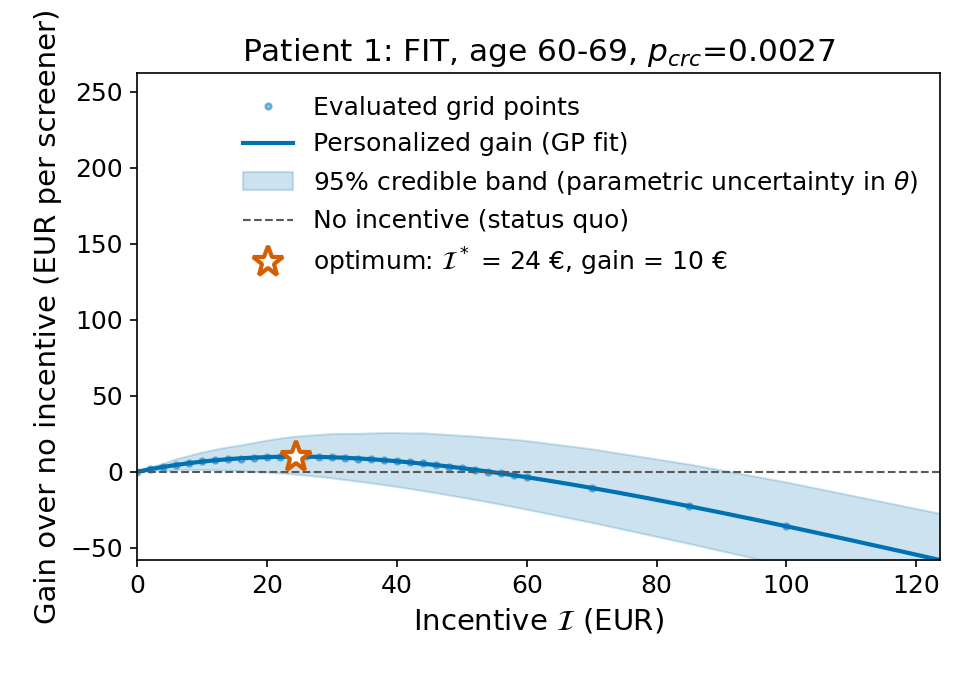
\includegraphics[width=\linewidth]{optimal_incentive_patient_1.png}
    \end{minipage}
    \begin{minipage}{0.325\textwidth}
        \centering
        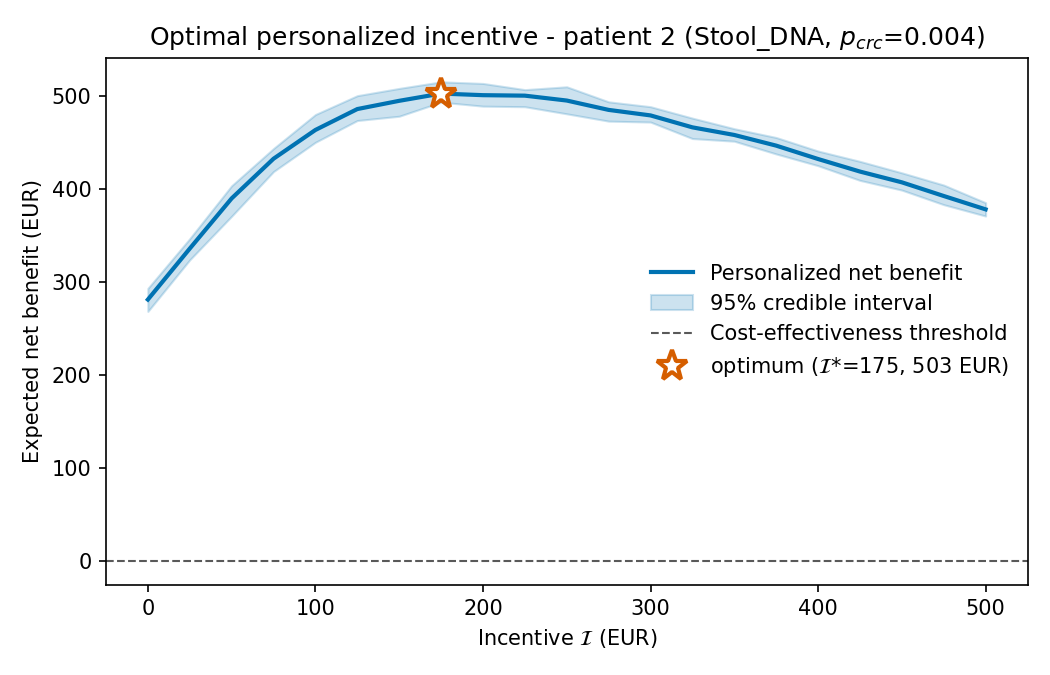
\includegraphics[width=\linewidth]{optimal_incentive_patient_2.png}
    \end{minipage}
    \begin{minipage}{0.325 \textwidth}
        \centering
        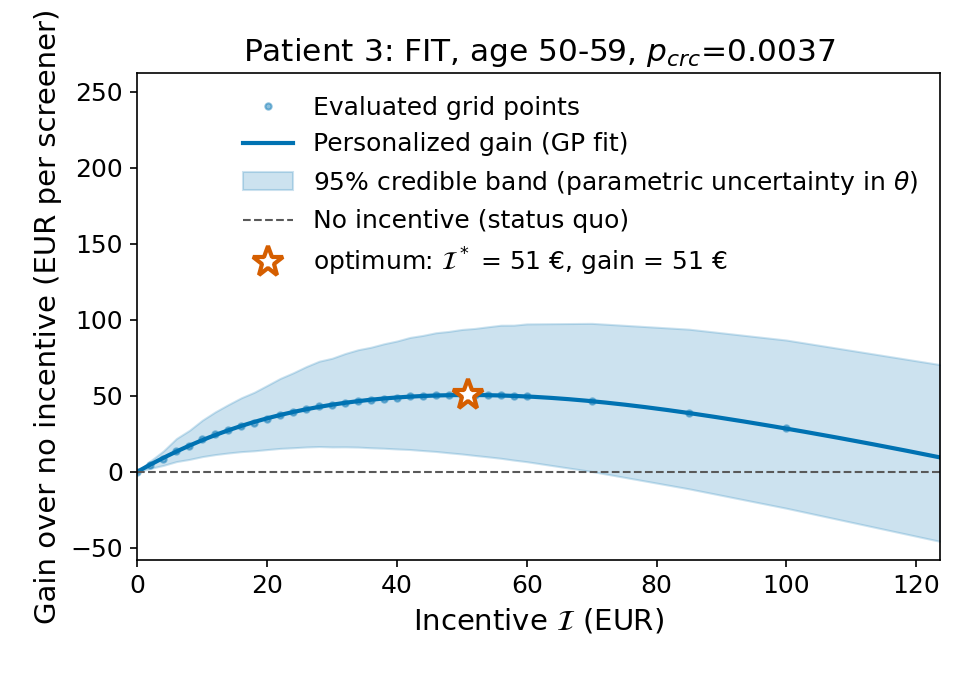
\includegraphics[width=\linewidth]{optimal_incentive_patient_3.png}
    \end{minipage}
    \caption{Optimal incentive for patients 1, 2 and 3. The dashed line at zero is the status quo, i.e.\ the same patient screened without any incentive.}
    \label{fig:images_experiments}
\end{figure}

Table~\ref{tab:detection_gain} details the role of age in Section~\ref{sec:public_scheme_results}. The health value to the PM of detecting a cancer by screening rather than clinically, $(\bar\delta_{\text{cli}} - \bar\delta_{\text{scr}})\, \big[V^{PM}_{\text{future}}(0,x) - V^{PM}_{\text{future}}(1,x)\big] + \mathbb{E}[V^{PM}_{\text{treat}}(g,x) \mid \text{clinical}] - \mathbb{E}[V^{PM}_{\text{treat}}(g,x) \mid \text{screen}]$, doubles from ages 60--69 to 20--29, because younger citizens have more life-years to lose; the second term, the quality of life spared by treating an earlier stage, is worth 3{,}030€ at 60--69 and 3{,}310€ at 20--29, scaling with the age group's health utility. Citizens perceive a smaller health value, discounted at $\lambda_C$ and weighted by present bias and risk perception, which also rises less steeply as age falls. Since the value of screening a citizen scales with their risk, however, and their risk falls faster with age than the value of a detection rises, younger citizens are both less valuable to screen and less willing to participate.
\begin{table}[h!]
\centering
\footnotesize
\caption{Health value of a screen-detected rather than clinically detected cancer, by age (€). Citizen: at $\lambda_C$, weighted by present bias and risk perception. Ratios relative to 60--69.}
\label{tab:detection_gain}
\begin{tabular}{c c r c r c}
\toprule
\textbf{Age} & $\bar{Y}(a)$ & \textbf{PM} & \textbf{Ratio} & \textbf{Citizen, perceived} & \textbf{Ratio} \\
\midrule
20--29 & 59.5 & 118{,}302 & 1.99 & 35{,}687 & 1.64 \\
30--39 & 49.7 & 109{,}164 & 1.84 & 34{,}194 & 1.57 \\
40--49 & 40.0 &  95{,}152 & 1.60 & 31{,}195 & 1.43 \\
50--59 & 30.65 & 78{,}325 & 1.32 & 27{,}071 & 1.24 \\
60--69 & 21.9 &  59{,}410 & 1.00 & 21{,}764 & 1.00 \\
\bottomrule
\end{tabular}
\end{table}


\bibliography{sample}

\end{document}
